\documentclass[12pt]{report}
\usepackage[utf8]{inputenc}     % for éô
\usepackage[english]{babel}     % for proper word breaking at line ends
\usepackage[a4paper, left=1.4in, right=1.2in, top=1.3in, bottom=1.3in]{geometry}
                                % for page size and margin settings
\usepackage{graphicx}           % for ?
\usepackage{amsmath,amssymb}    % for better equations
\usepackage{amsthm}             % for better theorem styles
\usepackage{mathtools}          % for greek math symbol formatting
\usepackage{enumitem}           % for control of 'enumerate' numbering
\usepackage{listings}           % for control of 'itemize' spacing
\usepackage{todonotes}          % for clear TODO notes
\usepackage{hyperref}           % page numbers and '\ref's become clickable
\usepackage{setspace}
\usepackage{titlesec}
\usepackage{subfig}

%for aligning images
\usepackage[export]{adjustbox}
\usepackage{multirow}
\usepackage{xcolor}
\usepackage{hhline}
\usepackage{colortbl}
\usepackage{wrapfig}

% For quoting code
\definecolor{verde}{rgb}{0.25,0.5,0.35}
\definecolor{jpurple}{rgb}{0.5,0,0.35}
\definecolor{darkgreen}{rgb}{0.0, 0.2, 0.13}
\definecolor{oldmauve}{rgb}{0.4, 0.19, 0.28}
\newcommand{\python}{
  \lstset{ %
    language=Python,                % the language of the code
    basicstyle=\footnotesize,       % the size of the fonts that are used for the code
    numbers=left,                   % where to put the line-numbers
    numberstyle=\tiny\color{gray},  % the style that is used for the line-numbers
    stepnumber=1,                   % the step between two line-numbers. If it's 1, each line
                                    % will be numbered
    numbersep=5pt,                  % how far the line-numbers are from the code
    backgroundcolor=\color{white},  % choose the background color. You must add \usepackage{color}
    showspaces=false,               % show spaces adding particular underscores
    showstringspaces=false,         % underline spaces within strings
    showtabs=false,                 % show tabs within strings adding particular underscores
    frame=single,                   % adds a frame around the code
    rulecolor=\color{black},        % if not set, the frame-color may be changed on line-breaks within not-black text (e.g. commens (green here))
    tabsize=2,                      % sets default tabsize to 2 spaces
    captionpos=b,                   % sets the caption-position to bottom
    breaklines=true,                % sets automatic line breaking
    breakatwhitespace=false,        % sets if automatic breaks should only happen at whitespace
    title=\lstname,                 % show the filename of files included with \lstinputlisting;
                                    % also try caption instead of title
    keywordstyle=\color{blue},      % keyword style
    commentstyle=\color{darkgreen},   % comment style
    stringstyle=\color{red},      % string literal style
    escapeinside={\%*}{*)},         % if you want to add a comment within your code
    morekeywords={*,...}          % if you want to add more keywords to the set
}}

\colorlet{punct}{red!60!black}
\definecolor{background}{HTML}{EEEEEE}
\definecolor{delim}{RGB}{20,105,176}
\colorlet{numb}{magenta!60!black}

\lstdefinelanguage{json}{
    basicstyle=\normalfont\ttfamily,
    numbers=left,
    numberstyle=\scriptsize,
    stepnumber=1,
    numbersep=8pt,
    showstringspaces=false,
    breaklines=true,
    frame=lines,
    backgroundcolor=\color{background},
    literate=
     *{0}{{{\color{numb}0}}}{1}
      {1}{{{\color{numb}1}}}{1}
      {2}{{{\color{numb}2}}}{1}
      {3}{{{\color{numb}3}}}{1}
      {4}{{{\color{numb}4}}}{1}
      {5}{{{\color{numb}5}}}{1}
      {6}{{{\color{numb}6}}}{1}
      {7}{{{\color{numb}7}}}{1}
      {8}{{{\color{numb}8}}}{1}
      {9}{{{\color{numb}9}}}{1}
      {:}{{{\color{punct}{:}}}}{1}
      {,}{{{\color{punct}{,}}}}{1}
      {\{}{{{\color{delim}{\{}}}}{1}
      {\}}{{{\color{delim}{\}}}}}{1}
      {[}{{{\color{delim}{[}}}}{1}
      {]}{{{\color{delim}{]}}}}{1},
}


% Removes indentation of paragraphs
\usepackage{parskip}
\setlength{\parskip}{1em}

% Formatting for the paging styles
\usepackage{fancyhdr}
\pagestyle{fancy}
\fancyhf{}
\fancyhead[L]{\leftmark}
\fancyhead[R]{\thepage}

% The sizing of the section text
\titleformat*{\section}{\LARGE\bfseries}
\titleformat*{\subsection}{\Large\bfseries}
\titleformat*{\subsubsection}{\large\bfseries}

% Formatting for the individual chapters
\titleformat{\chapter}[display]
    {\normalfont\huge\bfseries}{\chaptertitlename\ \thechapter}{20pt}{\Huge}
\titlespacing*{\chapter}{0pt}{0pt}{35pt}

% Display References instead of Bibliography
\addto\captionsenglish{\renewcommand{\bibname}{References}} 

\onehalfspacing


%%%%%%%%%%%%%%%%%%%%%%%%%%%%%%%%
%% SET TITLE PAGE VALUES HERE %%
%%%%%%%%%%%%%%%%%%%%%%%%%%%%%%%%
%             ||               %
%             ||               %
%             \/               %

\def\thesistitle{Task Board Interpretation from Photographs}
\def\thesisauthorfirst{Richard-Johnson}
\def\thesisauthorsecond{Farukh}
\def\thesissupervisorfirst{Dr. Tim}
\def\thesissupervisorsecond{Morris}
\def\thesisdate{April 2019}



%% FOR PDF METADATA
\title{\thesistitle}
\author{\thesisauthorfirst\space\thesisauthorsecond}
\date{\thesisdate}

%% TODO PACKAGE
\newcommand{\towrite}[1]{\todo[inline,color=yellow!10]{TO WRITE: #1}}

%% THEOREM STYLES
\newtheorem{theorem}{Theorem}[section]
\newtheorem{corollary}{Corollary}[theorem]
\newtheorem{lemma}[theorem]{Lemma}
\newtheorem{proposition}[theorem]{Proposition}

\theoremstyle{definition}
\newtheorem{definition}[theorem]{Definition}

\theoremstyle{remark}
\newtheorem*{remark}{Remark}


%% MATH OPERATORS
\DeclareMathOperator{\supersine}{supersin}
\DeclareMathOperator{\supercosine}{supercos}

%%%%%%%%%%%%%%%%%%%%%%%

\begin{document}
\begin{titlepage}
	\thispagestyle{empty}
	\newcommand{\HRule}{\rule{\linewidth}{0.5mm}}
	\center
	\textsc{\Large The University of Manchester}\\[.7cm]
	
\includegraphics[width=25mm]{Crest_fullcolour.jpg}\\[.5cm]
	\textsc{School of Computer Science}\\[0.5cm]
	
	\HRule \\[0.4cm]
	{ \huge \bfseries \thesistitle}\\[0.1cm]
	\HRule \\[.5cm]
	\textsc{\large Third Year Project}\\[.5cm]
	
	\begin{minipage}{0.4\textwidth}
	\begin{flushleft} \large
	\emph{Author:}\\
	\thesisauthorfirst\space \textsc{\thesisauthorsecond}
	\end{flushleft}
	\end{minipage}
	~
	\begin{minipage}{0.4\textwidth}
	\begin{flushright} \large
	\emph{Supervisor:} \\
	\thesissupervisorfirst\space \textsc{\thesissupervisorsecond} \\[1em]
	\end{flushright}
    \end{minipage}\\[4cm]
    \normalsize{Submitted in partial fulfillment for the degree of}\\[0.1cm]
    \normalsize{BSc (Hons) in Computer Science with Industrial Experience}\\[0.5cm]
	\vfill
	{\large \thesisdate}\\
	\clearpage
\end{titlepage}

\chapter*{Abstract}
Task boards, and more specifically their Kanban standard, are a staple of organizational management and play a vital role in development teams. They are an intuitive way of interacting with tasks, viewing progress and tracking day-to-day activities. They allow project managers to extract useful information about their team's performance at a glance and serve as a subject matter in daily stand up meetings in agile teams.

But this method is not without its faults. The strictly physical presence does not provide automated analytics, a history, or reports of any mistakes and deficiencies. Having the Kanban board as a physical mirror of an established software solution introduces the possibility for inconsistencies and adds a risk of possible redundancy, which in turn could frustrate developers. 

This project aims to fuse the physical entity with the software equivalent using a pointed camera, computer vision and a NoSQL database in order to make changes to a project tracking service through a RESTful API, whilst trying to maintain the simplicity of using custom handwritten tickets, as opposed to purely native printed ones.
%%%%%%%%%%%%%%%%%%%%%%% 

\tableofcontents
\listoffigures
%%%%%%%%%%%%%%%%%%%%%%%

% EXAMPLES 

% \begin{definition}\label{def:domain}
% \begin{itemize}

% \end{itemize}
% \end{definition}

% \towrite{an introduction and some examples}

% \begin{theorem}[]
% \end{theorem}

% \begin{remark}
% \cite{Rynne2008LinearAnalysis}.
% \end{remark}


% \begin{figure}[h]
%     \centering
%     
\includegraphics[width=.3\textwidth]{Crest_fullcolour.jpg}
%     \caption{Motivational illustration. Similar to \cite{Oort1958,Reed1960}.}
%     \label{fig:logo}
% \end{figure}

% \begin{corollary}
% \end{corollary}

% The proof of this theorem is illustrated in Figure \ref{fig:logo}.

% \begin{figure}
%     \centering
%     
\includegraphics[width=.7\textwidth]{Crest_fullcolour.jpg}
%     \caption{A cute dog.}
%     \label{fig:my_label}
% \end{figure}

% \begin{lstlisting}[language=json,firstnumber=1]
% {"menu": {
%     "id": "file",
%     "value": "File",
%     "popup": {
%         "menuitem": [
%         {"value": "New", "onclick": "CreateNewDoc()"},
%         {"value": "Open", "onclick": "OpenDoc()"},
%         {"value": "Close", "onclick": "CloseDoc()"}
%         ]
%     }
% }}
% \end{lstlisting}

% \begin{lstlisting}[language=bash]
%     $ wget http://tex.stackexchange.com
%   \end{lstlisting}

%%%%%%%%%%%%%%%%%%%%%%%

\newpage
\chapter{Introduction}
\section{Background}

The motivations for this project sprawled from observing an inherent flaw in the working pipeline of most software development teams. In examining the current process of the interaction with project tracking software as well as the task boards, which are their physical representation, there was an apparent deficiency, which this project aims to solve.

The issues were first encountered whilst being on an industrial placement. After experiencing countless problems with the conventional methodology, the inherent flaw became self-evident, which was the time that the idea for the project initially grew its roots.

Undeniably, there are fully digital solutions which make the project redundant, but the physical task board has stood the test of time, and interfacing with a physical entity as opposed to software is always found preferable when there is a degree of dimensionality. In this example, that degree is the movement of physical tickets across a 2D plane.

\section{Task board}
In the software development industry, individual teams ordinarily employ physical task boards, which the use Kanban. Kanban is a scheduling system for lean, just-in-time manufacturing, which was originally developed to improve manufacturing efficiency. 

Software development teams use these task boards as a guide for productivity and as a visual aid, which is kept up-to-date with the online project tracking software by the developers working on the projects they represent.

The boards themselves contain tickets, which could be issues, bugs or features that a current project might contain, and they are visually segmented into sections, with each section representing a state that a ticket could be in. A ticket changes states by being physically moved from one section of the board to another by a member of the team, and it can be assigned to that team member by them placing an associated tag containing their name on the ticket.

The boards themselves usually have workflow rules and limits, which should restrict the developers from exhibiting undesirable behavior, however, it is difficult for them to be enforced without the need for constant supervision of undergoing processes.

\section{Project tracking service}
The task board can be seen as a supplementary physical entity for the true underlying executor - the project tracking service (referred to simply as \textit{service}). The service itself features a database containing the issues, bugs, and features, and it is the source from which they are drawn before being put on the physical task board. Tickets are originally written by the project manager and are put in an online database which the service provides.

Developers can pick up these tickets by assigning the tickets to themselves on the service, which prevents anyone else from working on them simultaneously and thus wasting valuable resources. The reason why the service exists complementary to the physical board is that it stores records of activities, comments, and provides statistical data relating to productivity.

Examples of such software: 

\begin{itemize}
    \item{\textbf{Todoist}\footnote{\url{https://todoist.com/}} - a to-do list application, with robust project management capabilities, which was primarily used for interfacing in this project}
    \item{\textbf{JIRA}\footnote{\url{https://www.atlassian.com/software/jira}} - a proprietary issue tracking product developed by Atlassian that allows bug tracking and agile project management}
    \item{\textbf{Trello}\footnote{\url{https://trello.com/en-GB}} - a web-based list-making application originally made by Fog Creek Software in 2011}
    \item{\textbf{Redmine}\footnote{\url{https://www.redmine.org/}} - is a free and open source, web-based project management and issue tracking tool}
\end{itemize}

\section{Justification}
A problem arises when we realize that the task board and the digital project tracker are two separate disjointed entities, which are only interconnected by the people interacting with them. With that being the case, any synchronization between the two entities is going to be the responsibility of the developers using them. This simply introduces redundancy, as developers need to make the same changes on the service and on the board, which should only be a single action.

\subsection{Problems}
\label{subsec:problems}
\begin{itemize}
    \item A ticket is moved on the board without it changing states on the service
    \item A ticket is assigned without it changing states on the service
    \item A ticket is assigned to multiple people on the board
    \item A ticket is moved illegally with regards to the desired workflow
    \item A ticket on the board does not exist on the service
    \item The ticket limit is unknowingly reached for a section on the board 
\end{itemize}

\subsection{Proposed solution}
One possible solution to the problem is to have a camera in front of the task board, which either takes video or periodically takes photos to capture the current state. Then, given that data, using computer vision and the RESTful API\footnote{Representational State Transfer}\footnote{Application Programming Interface} of the service, the necessary information would be extracted from the individual frames in order to facilitate the translation of those changes from the photos to changes on the project tracking service.

The project uses an emulated board on paper with a vivid colored border, which sections are segmented using a different color. The tickets themselves are small post-it notes, which contain a discernable digit in their top portion. The tags for individual developers are cut out QR\footnote{Quick Response code} codes on paper. For reusability, the ticket limits for the sections are digits on paper cutouts. The photos are captured using a digital single-lens reflex camera, due to its variable focal length and sharp image output.

\section{Requirements}
\subsection{Functional requirements}
\subsubsection{As a developer:}
\begin{itemize}
    \item When I add a ticket to a section on the board, I would like it to change state on the service.
    \item When I move a ticket from one section to another on the board, I would like it to change state on the service.
    \item When I remove a ticket from the board, I would like it to keep its state on the service.
    \item When I place my tag on a ticket on the board, I would like it to get assigned to me on the service.
    \item When I remove my tag from a ticket on the board, I would like it to no longer be assigned to me on the service.
    \item When I place a ticket in-between several sections, I would like it to change state on the service to the one of the section where the majority of its area lies on the board.
\end{itemize}
\subsubsection{As a project manager:}
\begin{itemize}
    \item I would like the system to detect the board automatically without the need of manual interference.
    \item I would like the system to consistently identify and label the sections based on their size.
    \item I would like to be able to view the most recent changes to the board.
    \item I would like to be notified when multiple people are assigned to the same ticket.
    \item I would like to be notified when someone is working on multiple tickets.
    \item I would like to be alerted when the ticket limit of a section is reached or surpassed.
    \item I would like to be alerted when a ticket moves illegally with regards to the workflow.
    \item I would like to be alerted if a ticket on the board does not exist on the service.
    \item I would like to be able to restart the computer the service runs on without losing its state.
\end{itemize}
\subsection{Non-functional requirements}
\begin{itemize}
    \item The system needs to extract the information and perform the calculations fast enough to capture consecutive changes.
    \item The system needs to be deterministic (exhibit the same behavior when provided with the same input data).
    \item The system is aimed towards developers, and as such should provide a sufficient interface for the target user demographic.
    \item The system should handle exceptions and give sufficient feedback should it encounter any.
\end{itemize}

\section{Software dependencies}

\begin{itemize}
    \item{\textbf{Python 3.7.0} - an interpreted, high-level, general-purpose programming language, in which the majority of the project was written}
    \item{\textbf{pickle} - a built-in library which allows compressing of native python objects into a \textit{*.pkl} file}
    \item{\textbf{logging} - a built-in library that defines functions and classes which implement a flexible event logging system for applications and libraries}
    \item{\textbf{opencv-python}\footnote{\url{https://opencv-python-tutroals.readthedocs.io/en/latest/}} - a library that is designed to solve computer vision problems}
    \item{\textbf{NumPy}\footnote{\url{https://www.numpy.org/}}- a library that adds support for large, multi-dimensional arrays and matrices, along with a large collection of high-level mathematical functions to operate on these arrays}
    \item{\textbf{todoistAPI}\footnote{\url{https://developer.todoist.com/rest/v8/}} a RESTful API for interfacing with the Todoist application}
    \item{\textbf{pymongo} - a library containing tools for working with mongoDB
    \item \textbf{imutils}\footnote{\url{https://github.com/jrosebr1/imutils}} - a series of convenience functions to make basic image processing operations such as translation, rotation, resizing, skeletonization, and displaying Matplotlib images easier with OpenCV and Python}
    \item{\textbf{sklearn} - a free machine learning library for the Python programming language}
    \item{\textbf{Keras} - an open-source neural-network library written in Python}
    \item{\textbf{pyzbar} - a library for detecting and decoding barcodes and QR codes of different types}
\end{itemize}


\newpage
\chapter{Board Initialization}
\section{Equipment and setup}
Some specific equipment was required for creating the test images of the project. Given that access to a task board was necessary throughout development, a decision was made to instead use a personal miniature model, instead of a full-scale production one. This fact drives some of the design decisions, which will be explained in further detail.



\subsection{Camera}
The camera used was a Nikon d5100, which has a 16.2MP sensor with RAW\footnote{File format that captures all image data recorded by the sensor when you take a photo.} (NEF) image capture capabilities, however, the ones used by the program are 9.05MP JPG images, with the quality setting set to \textit{fine}. Most of the images shot were at a focal length between 25-75mm in order to minimize lens distortion, which was possible using the Nikkor 18-105mm VR zoom lens. The shots themselves were all taken at a locked focal range, with auto-focus and the stabilization of the lens being turned off, as the camera itself was stationed on a tripod and auto stabilization has been known to introduce small shakes when the camera is stationary.

\begin{figure}[h]
    \centering
    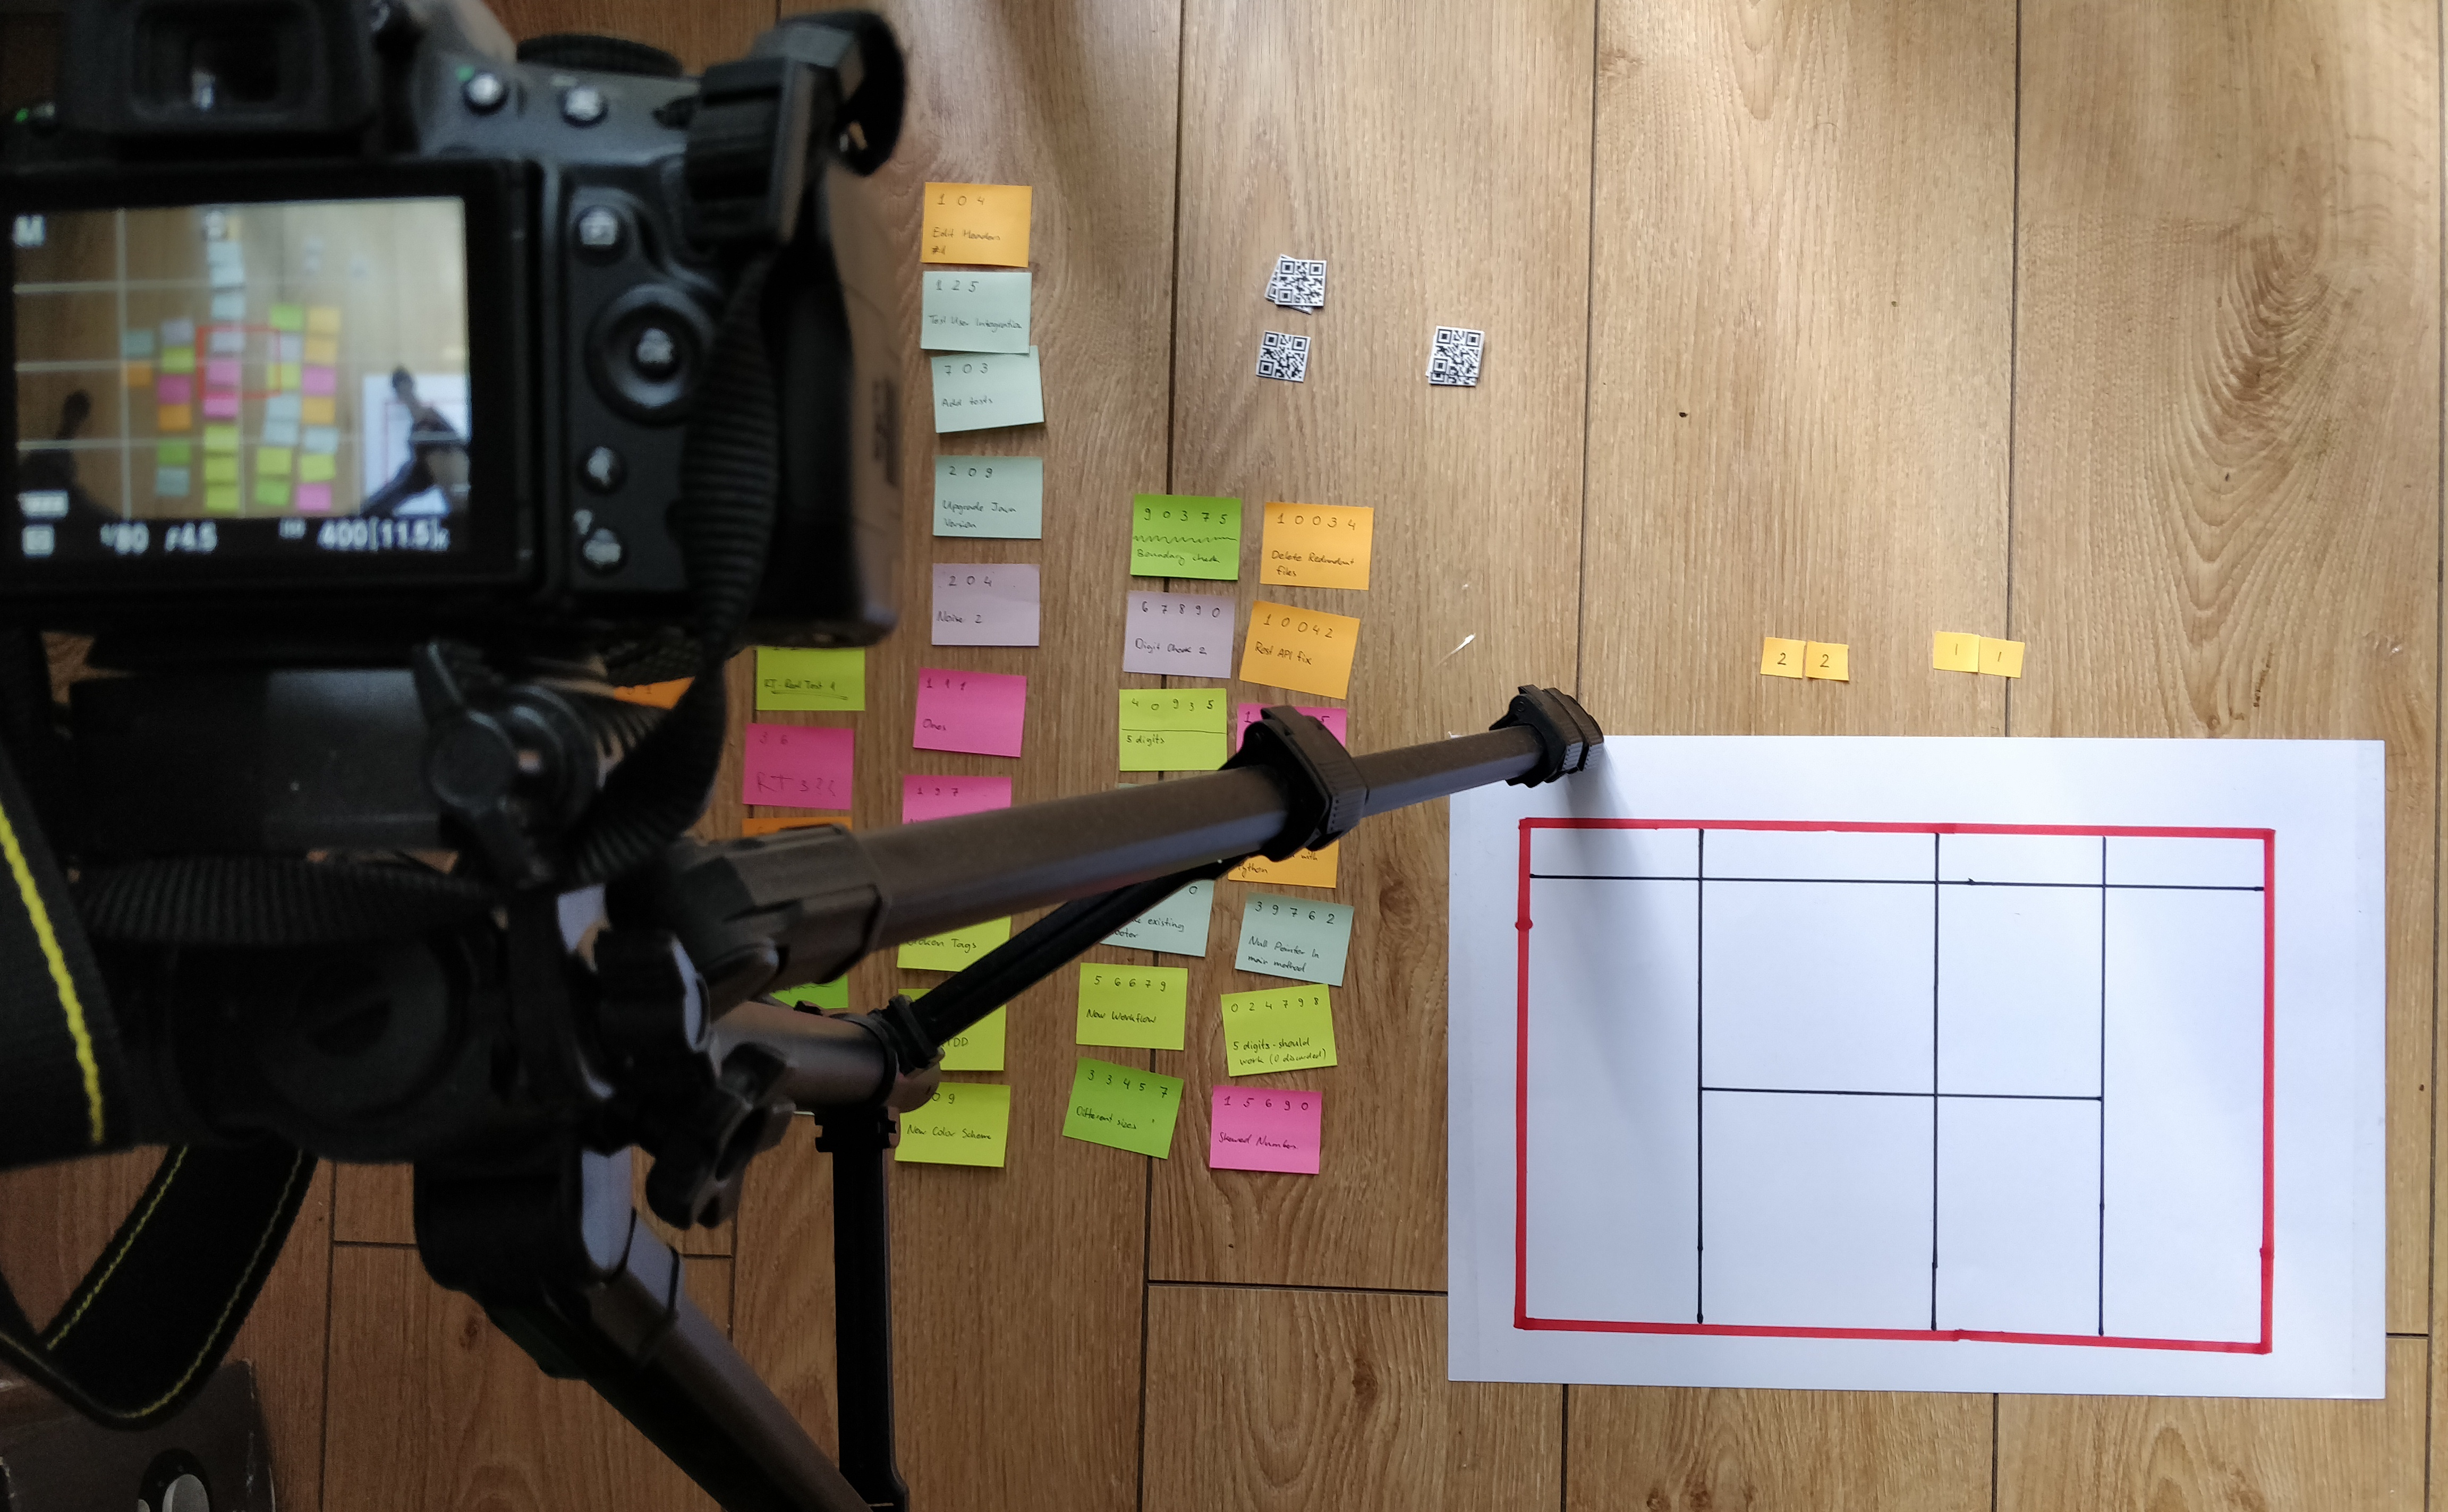
\includegraphics[width=\textwidth]{img/setup.jpg}
    \caption{Behind the scenes of image capture}
    \label{fig:setup}
\end{figure}

\subsection{Board}
The board itself was drawn on paper. It was meant to be a small-scale representation of the task board using a magnetic whiteboard. The border was meant to have colored masking tape, which in the small-scale model is just colored using a wide marker. The sections on a practical whiteboard would also be segmented using masking tape, and the small-scale model again used a marker to partition the task board. The original image of the board and the transformed and mapped one can both be seen in Figure \ref{fig:transformation}.

The top regions of the board were chosen to be either empty or as limits for the sections below them. On a real board, the limits would be written with a marker on the whiteboard itself, but as the development board needed to be reusable and is made of paper, the limits were digits written on paper cutouts and simply placed on top.

\begin{figure}%
    \centering
    \subfloat{{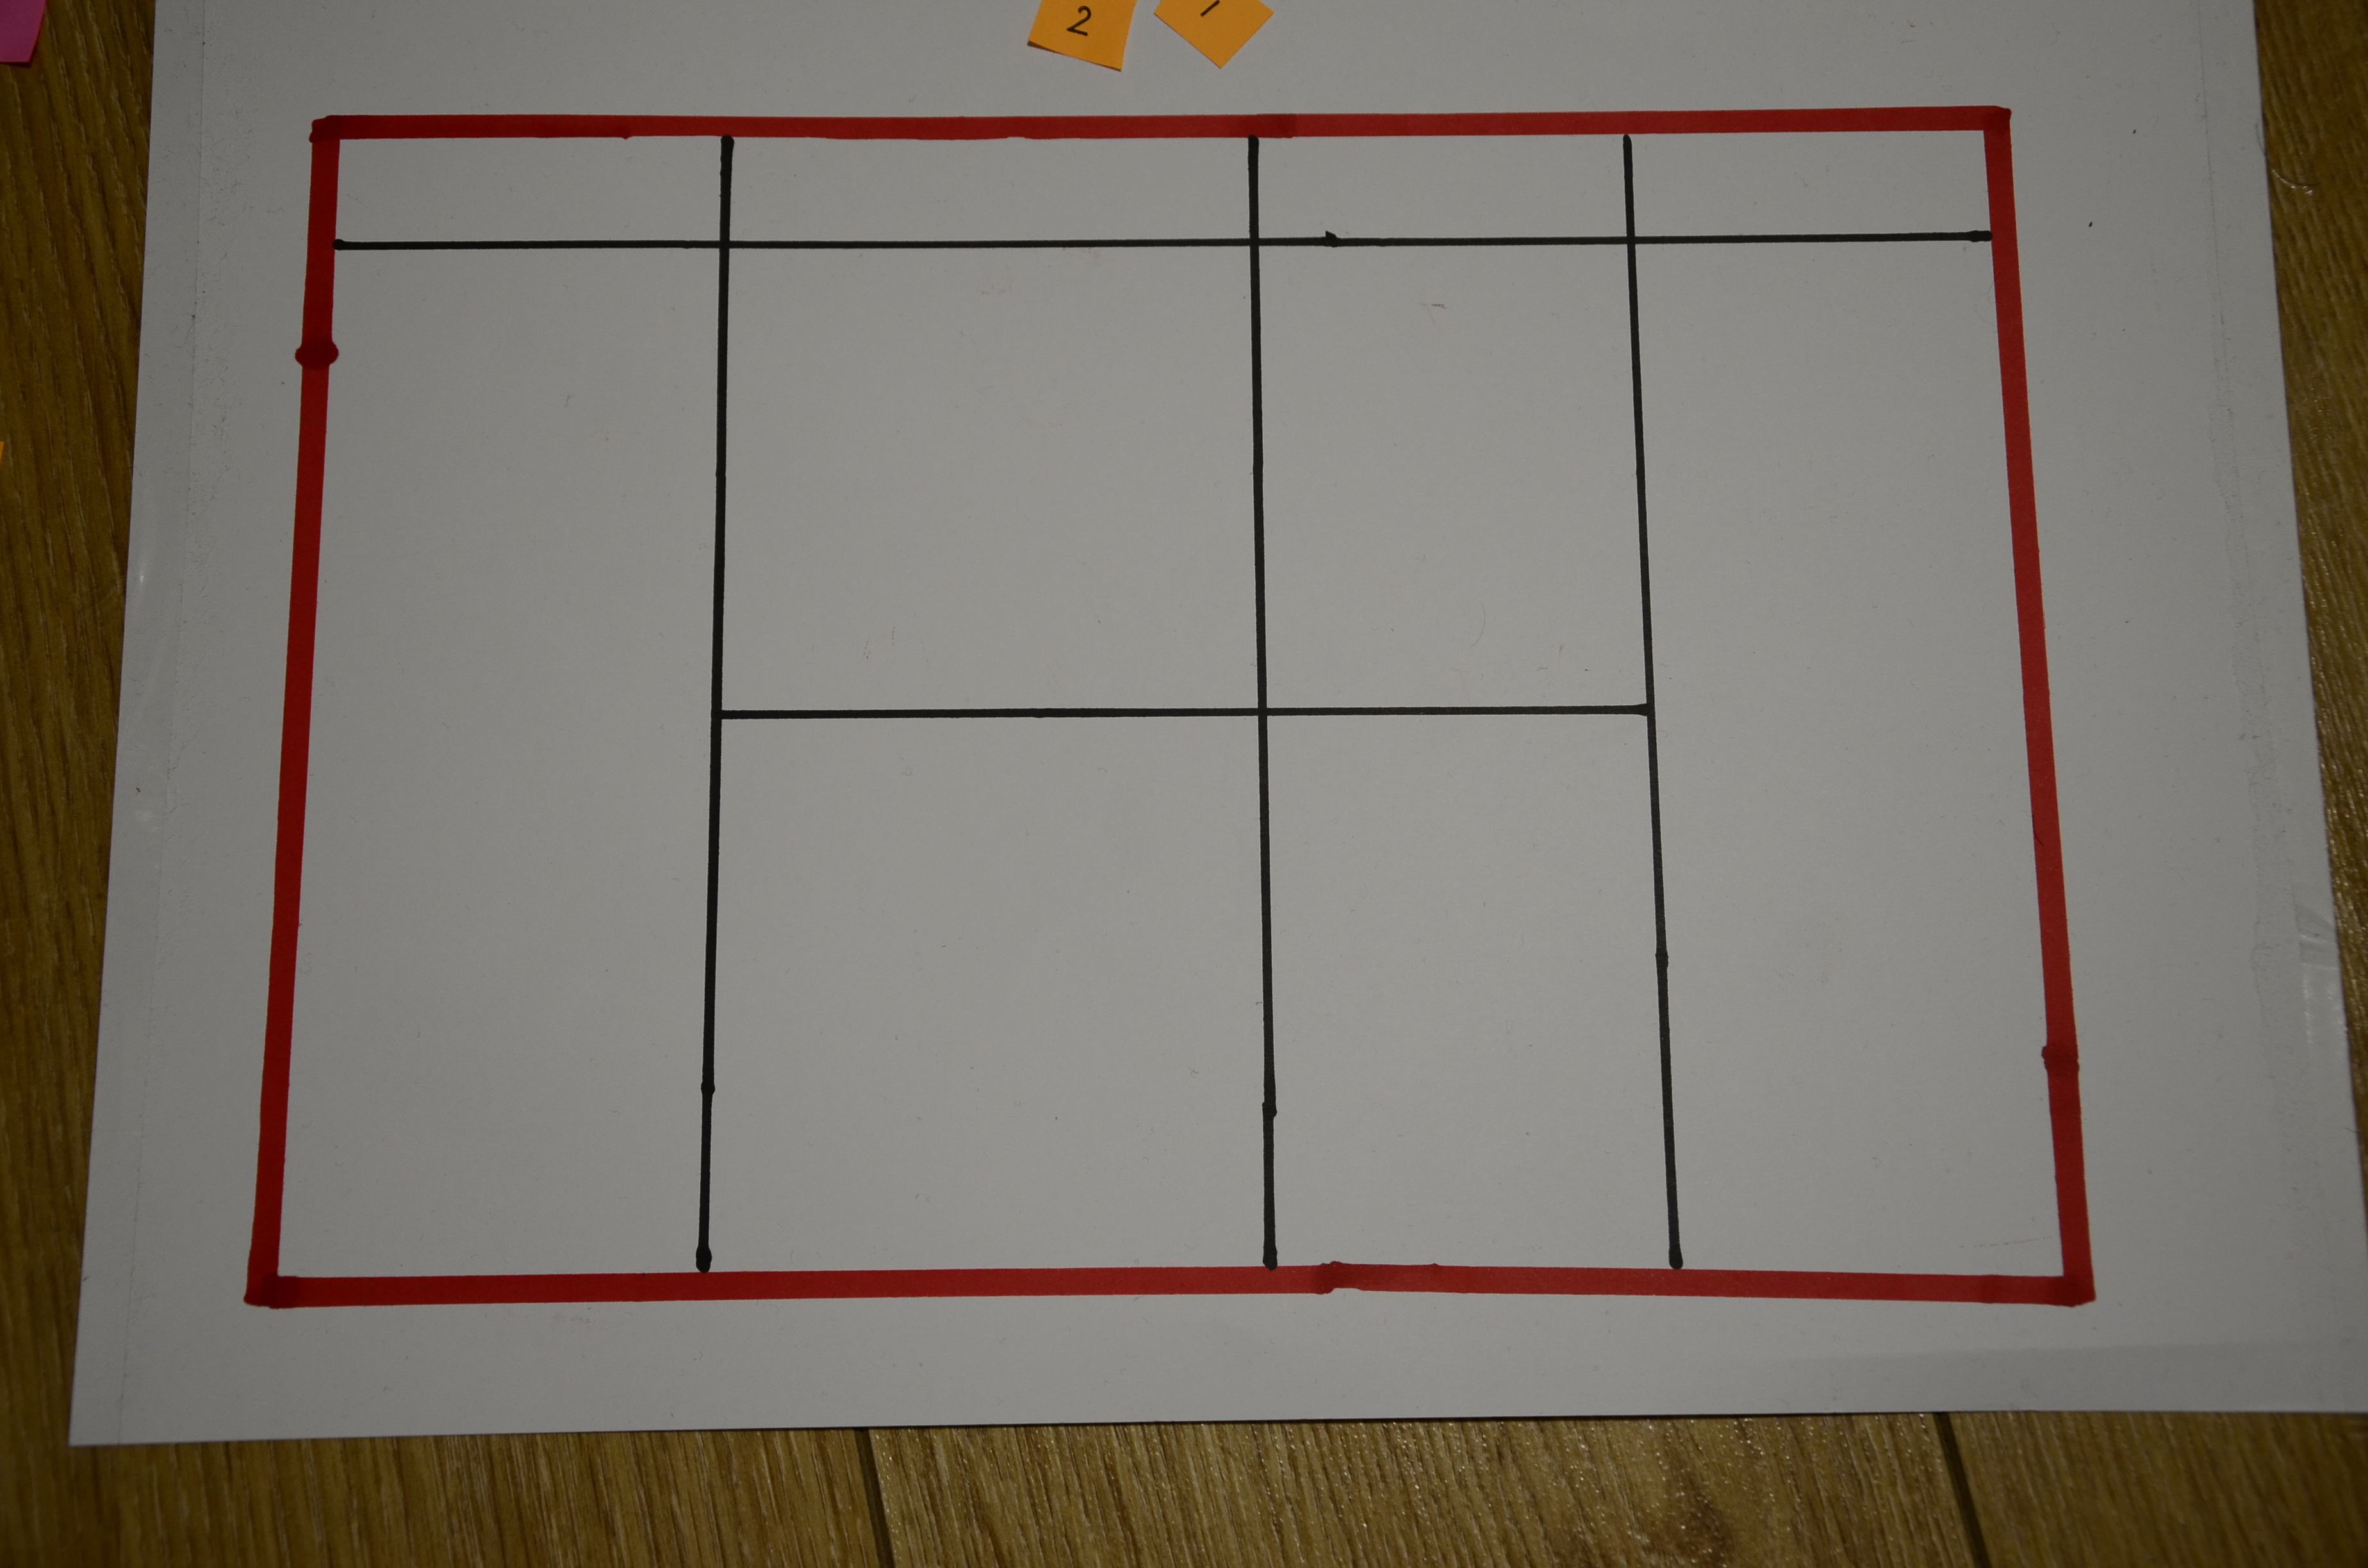
\includegraphics[width=\textwidth]{img/data/basic/_DSC7457.JPG}}}%
    \qquad
    \subfloat{{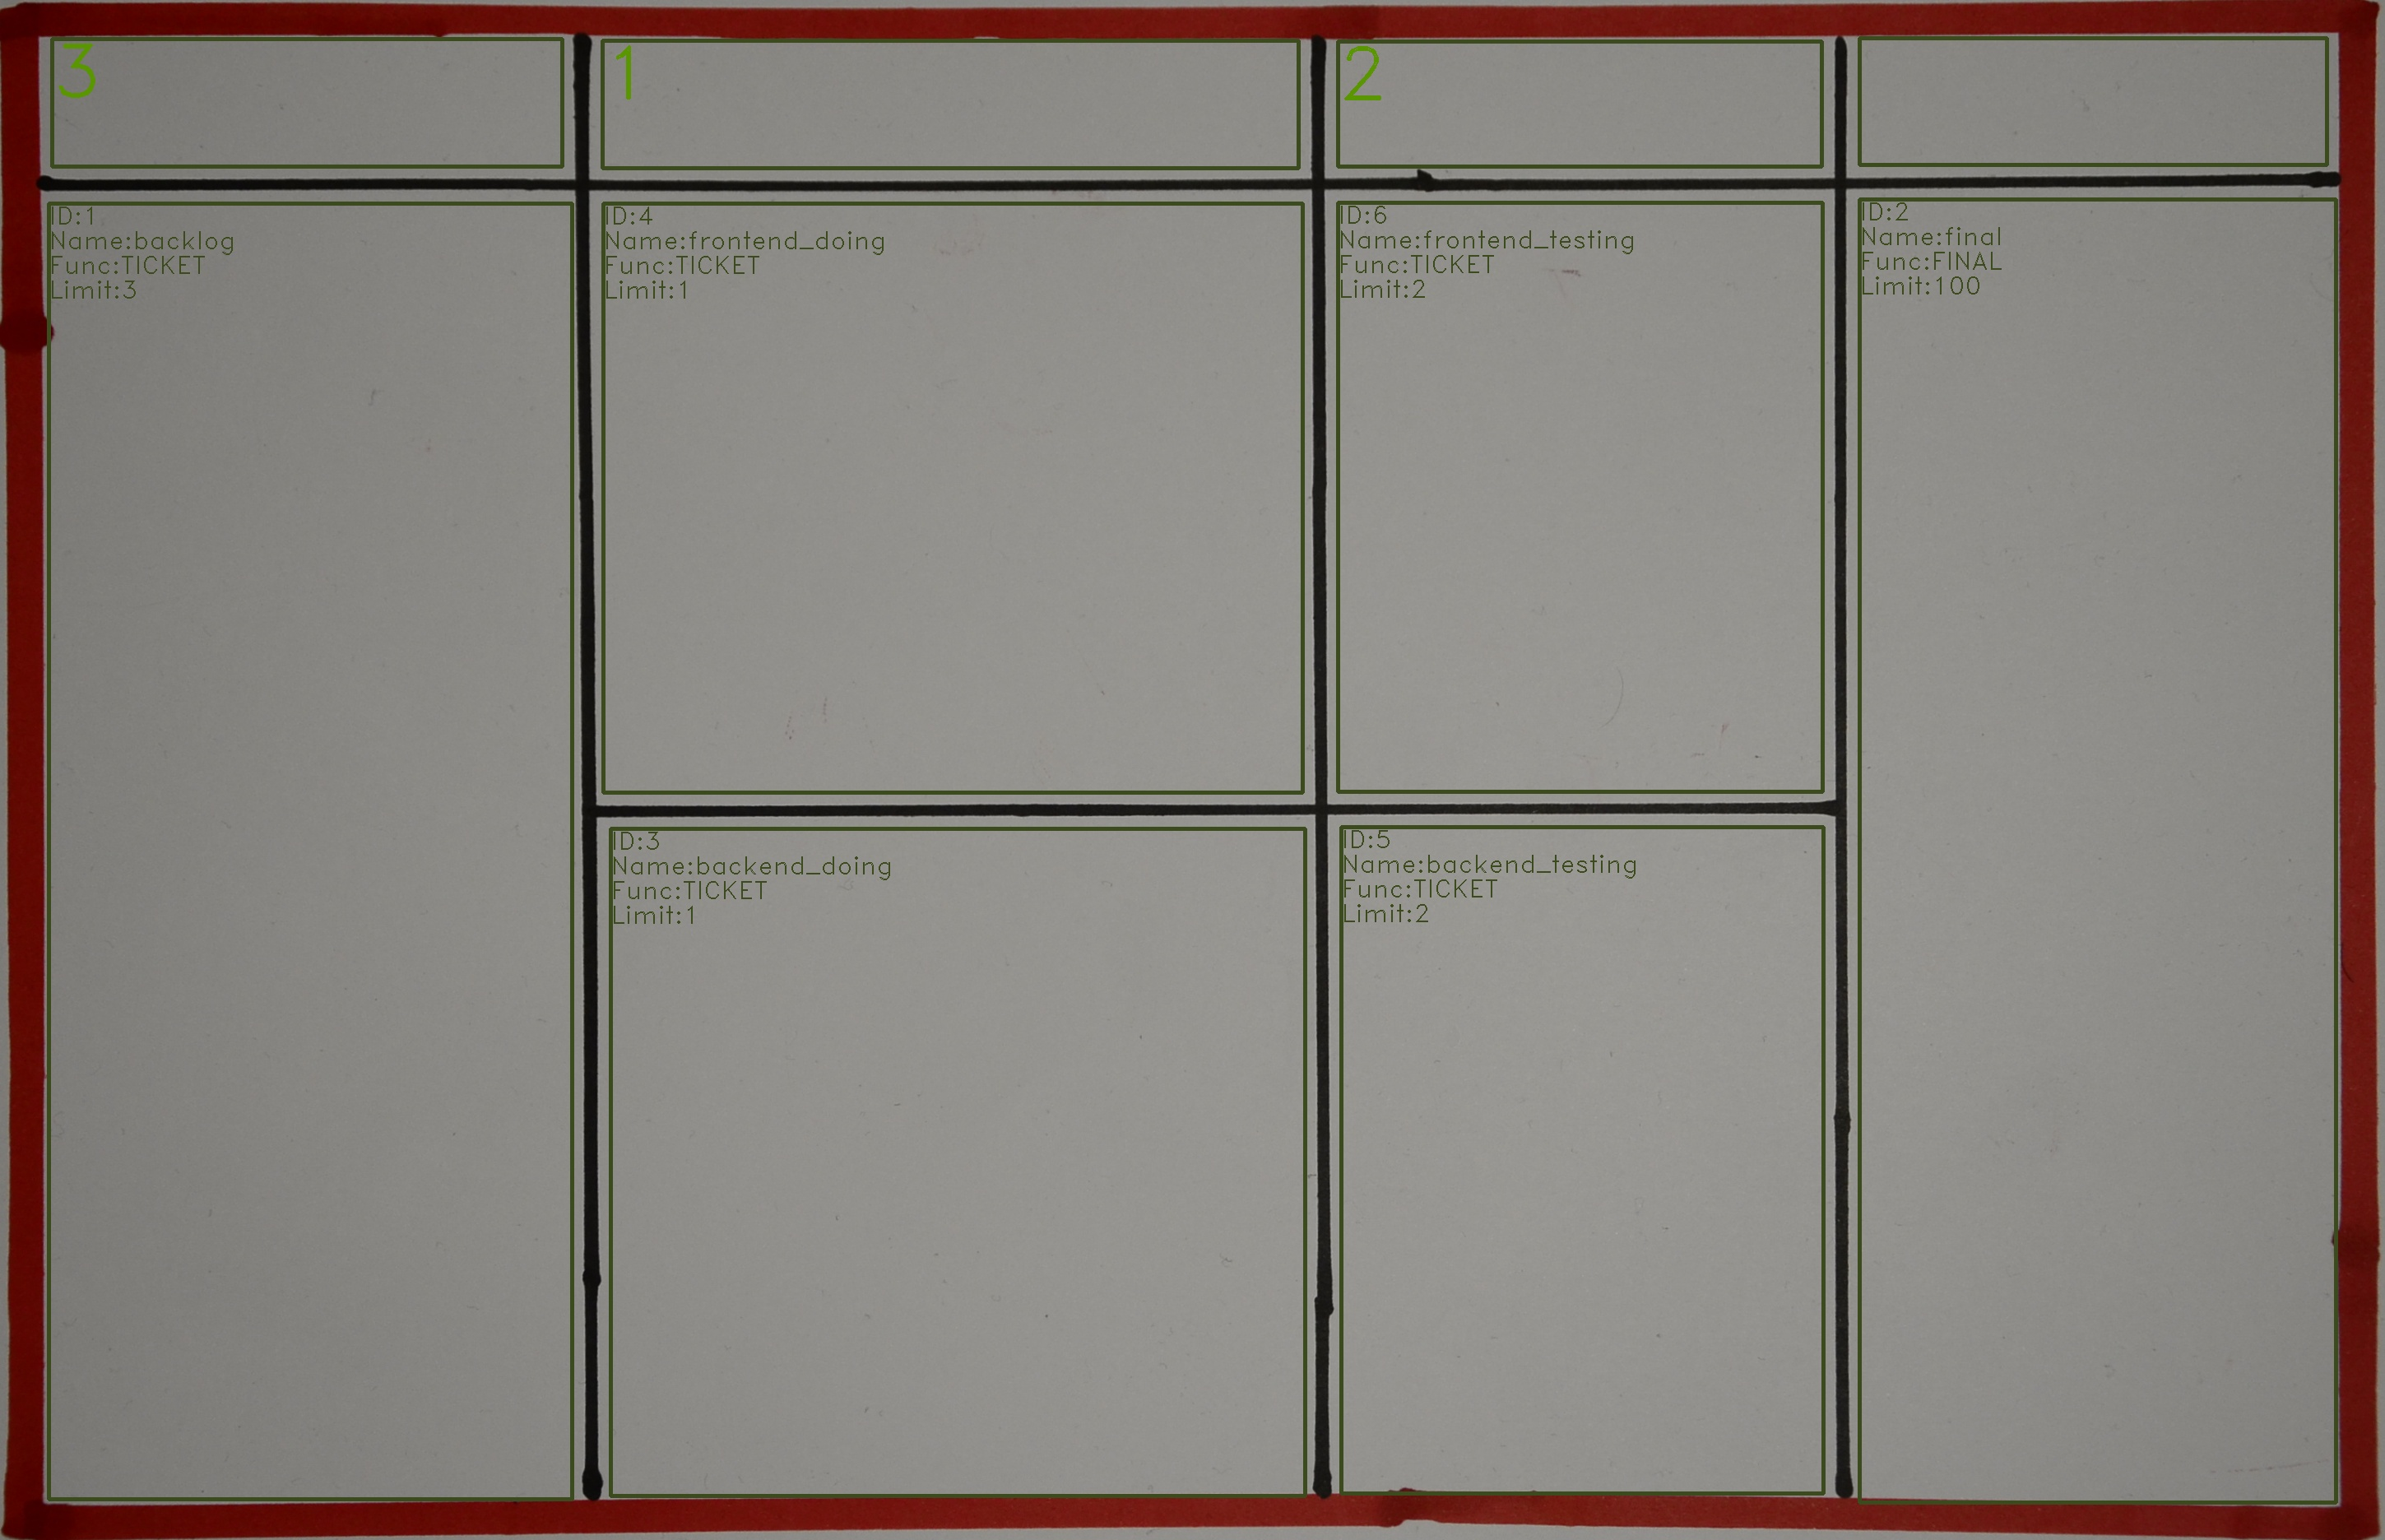
\includegraphics[width=\textwidth]{img/live_view/mapped_sections.jpg}}}%
    \caption{Original and transformed image}%
    \label{fig:transformation}%
\end{figure}

\subsection{Tickets}
The tickets are a key component in the overall equation, as they are the most common changes from image to image. They needed to be vibrant in color, in order to be distinguishable from the white background (the board) in incandescent lighting. Being vibrant, they also need to be contrasting the writing on them for legibility and scanning.

\begin{figure}[h]
    \centering
    \subfloat{{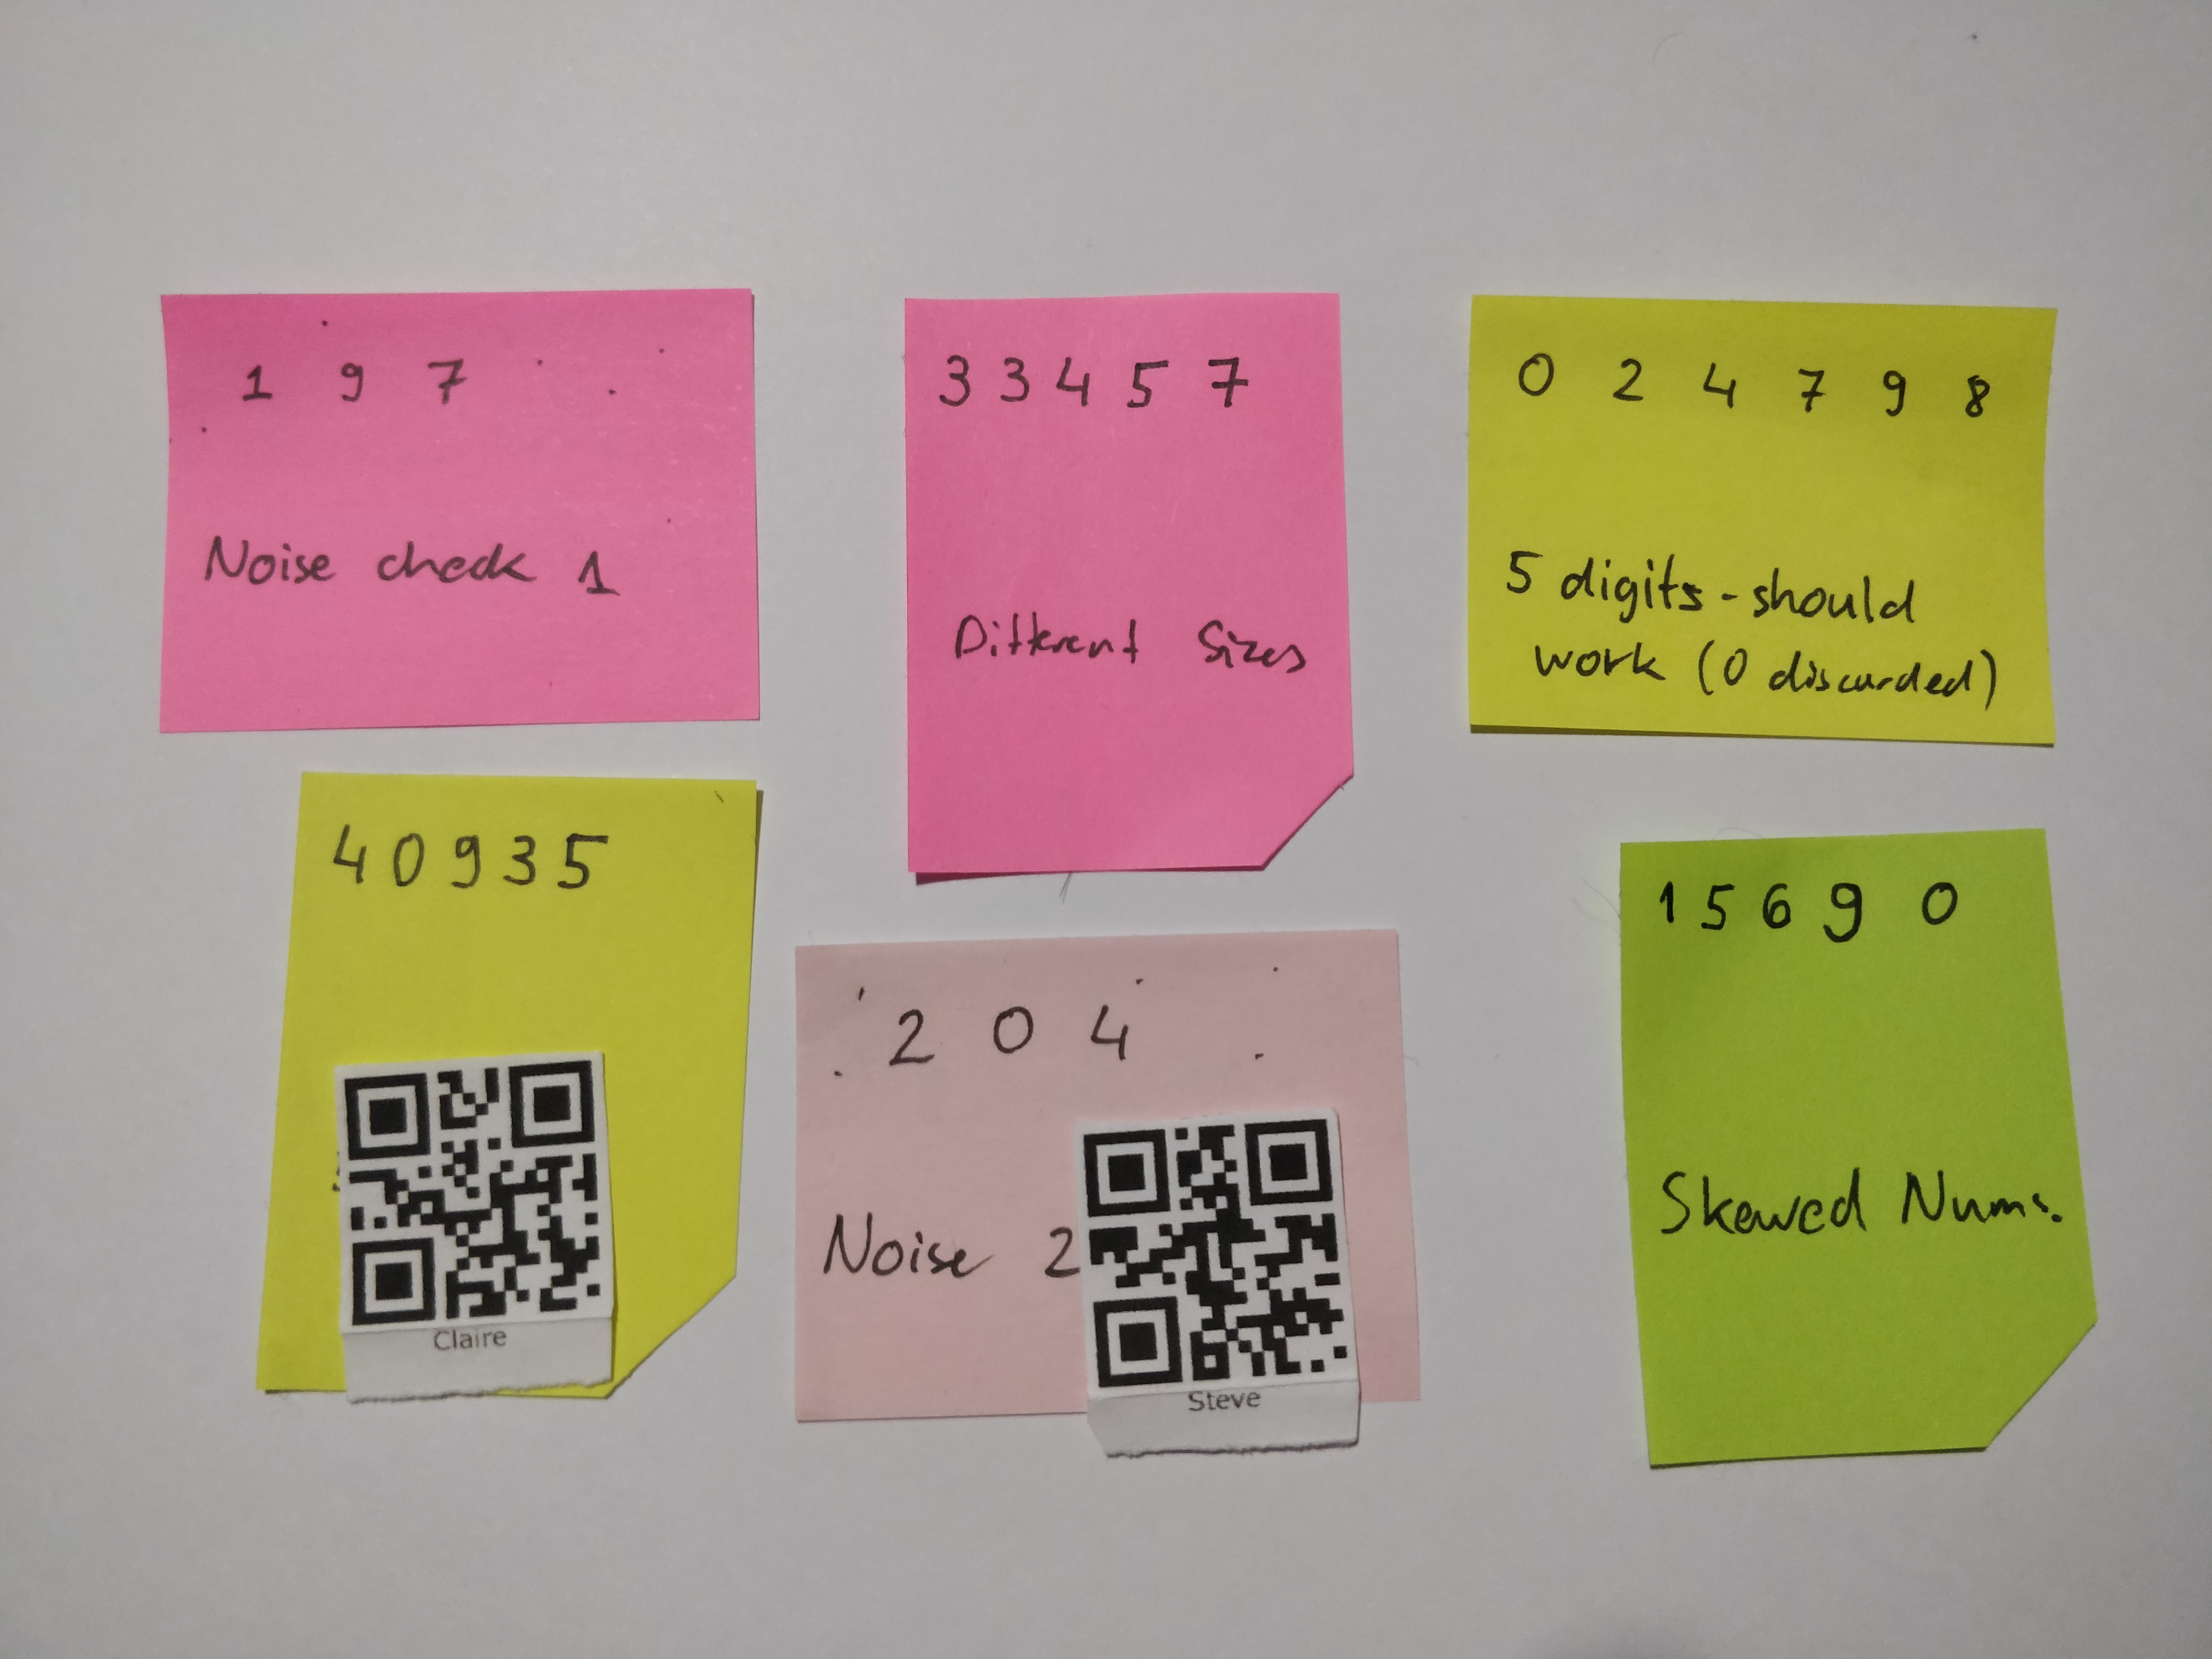
\includegraphics[height=5.5cm]{img/tickets_scale.jpg}}}
    \qquad
    \subfloat{{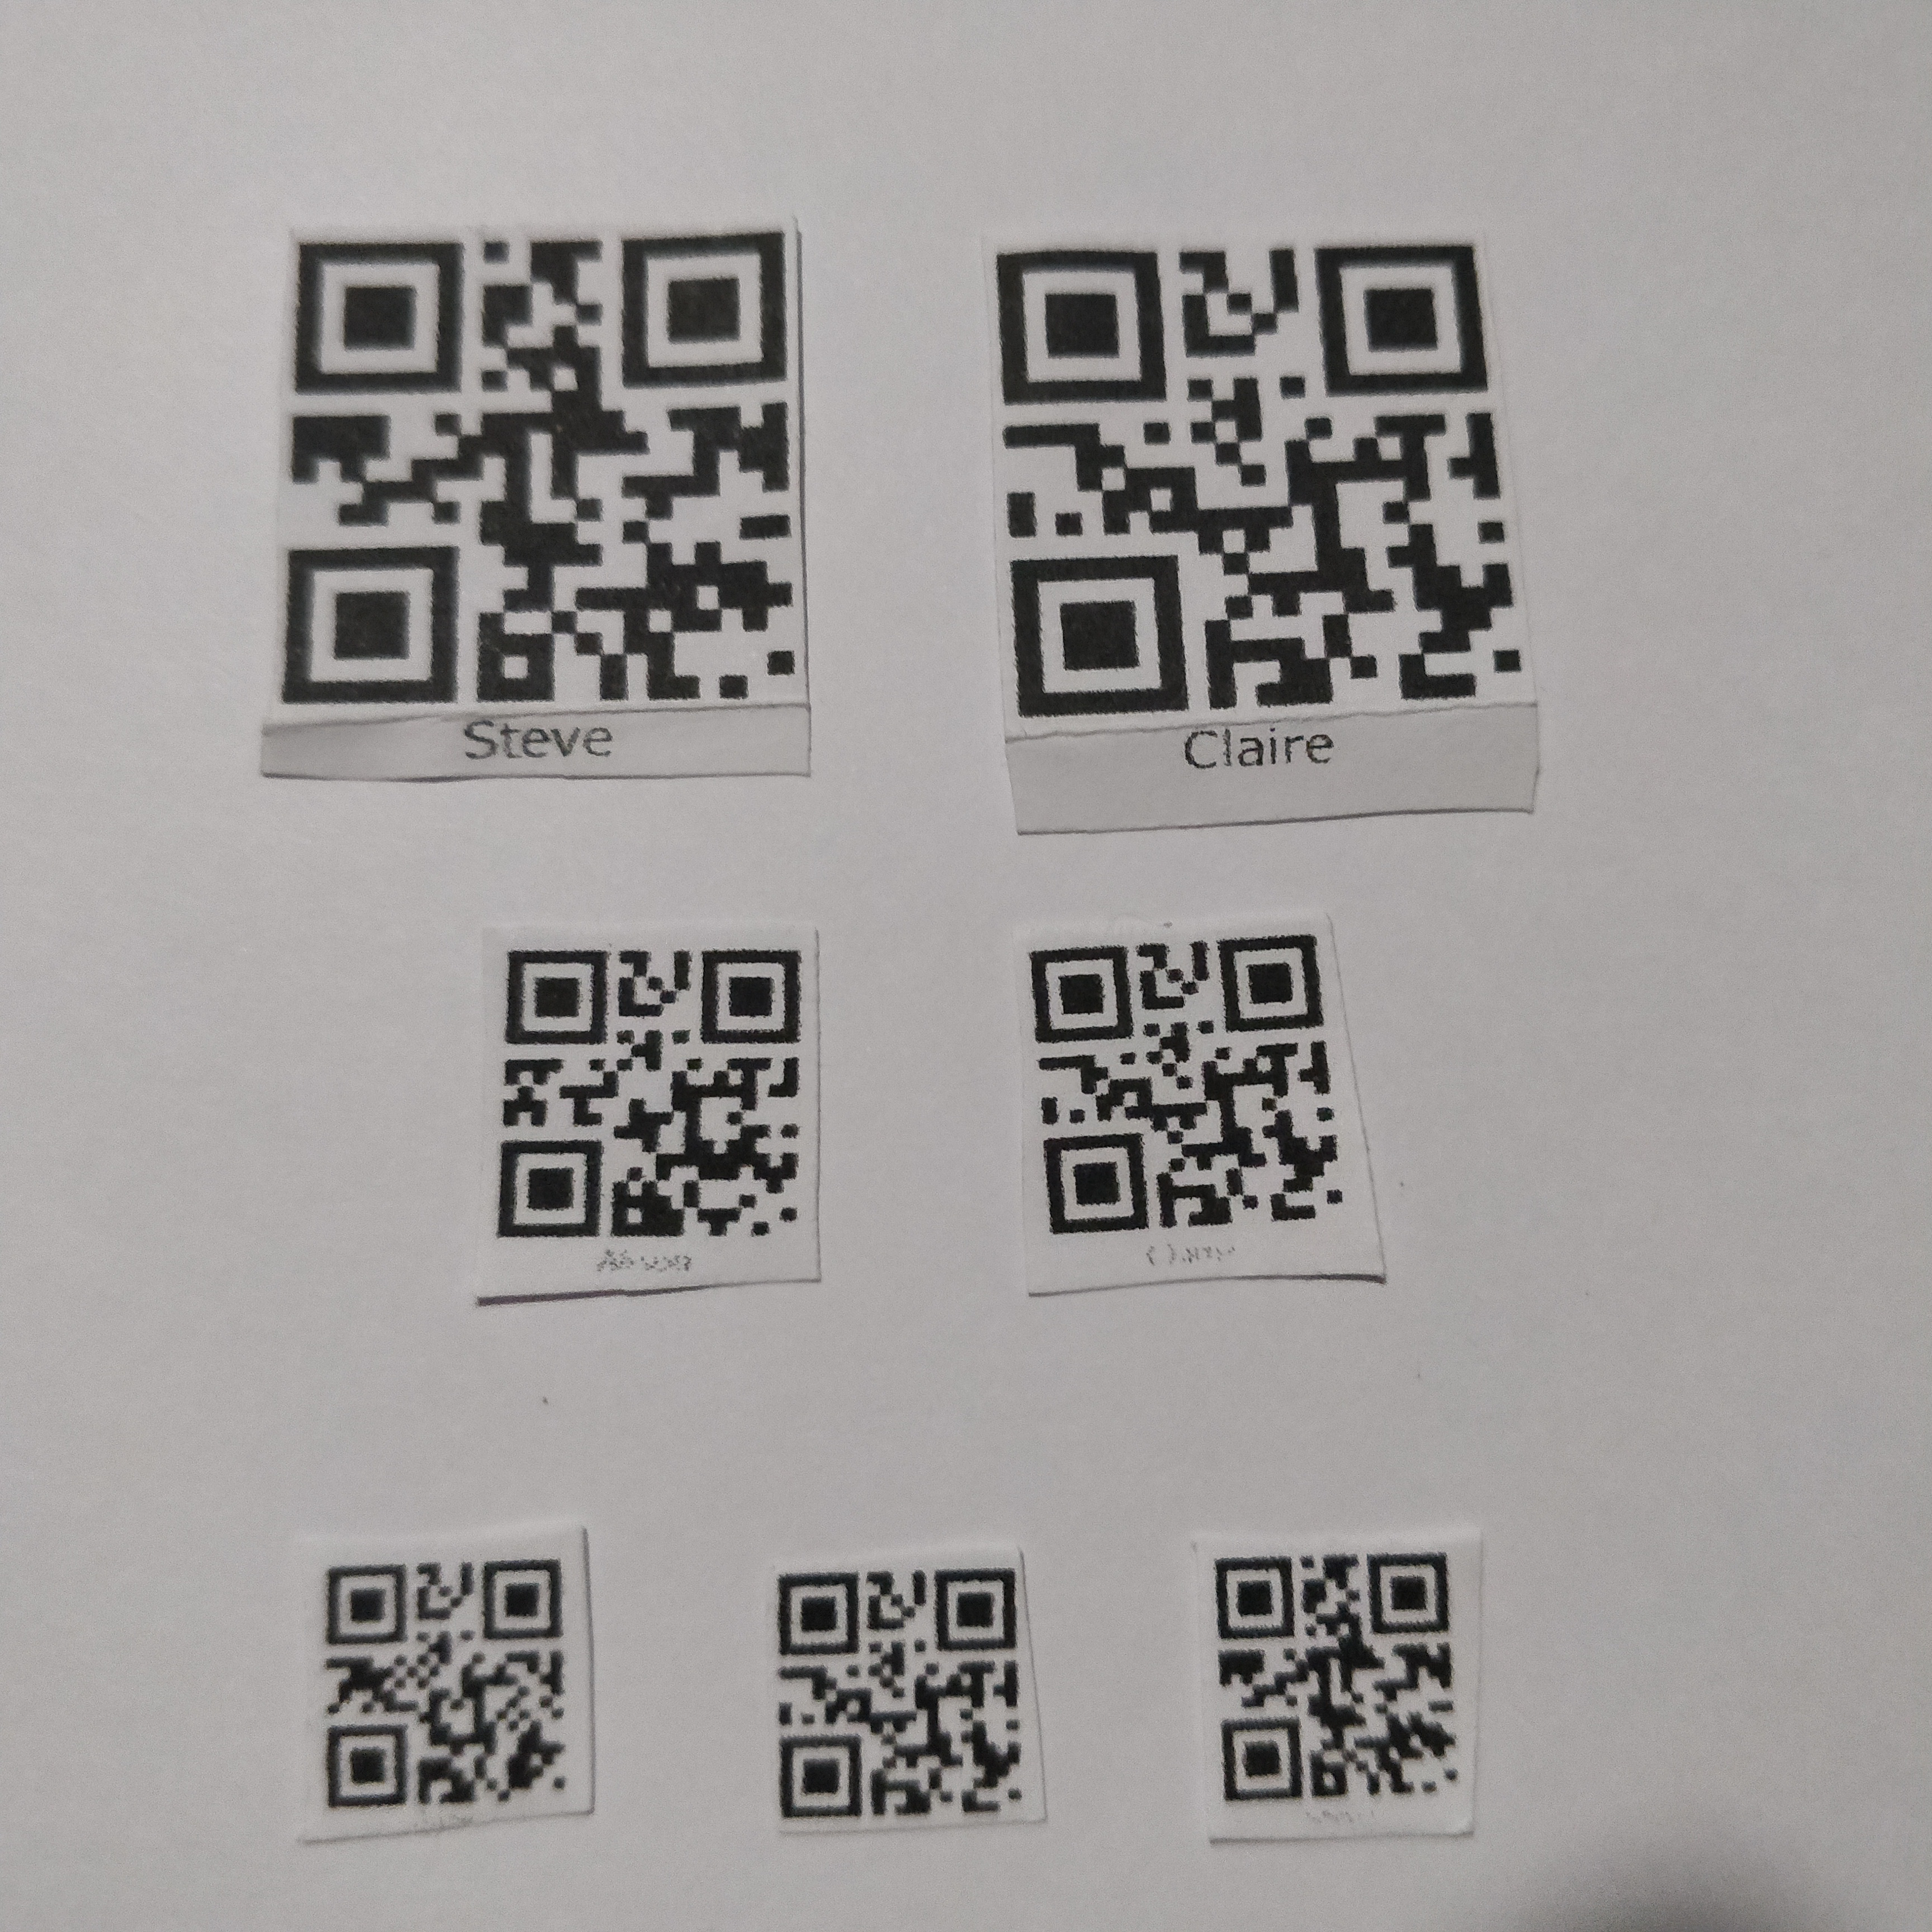
\includegraphics[height=5.5cm]{img/tags_scale.jpg}}}
    \caption{Tickets and experimental sizing for tag prints - 22 mm, 13 mm, 10 mm in width}
    \label{fig:tags_scale}
\end{figure}

The tickets themselves are adhesive post-it notes. The top portion of the ticket is scanned by the application in the ticket area itself, with the percentage occupied by the digit being adjustable in the settings file. The remaining bottom portion is reserved for writing the ticket description, which is strictly for the developers who read the tickets, as the application does not read the actual text on them (it already exists in the database). The bottom portion also serves as an area for placing the tags in such a way that they don't block the actual digits themselves.


\subsection{Tags}
In order to identify who assigned themselves to a ticket, there are special labels called \textbf{tags}, which are placed directly on the ticket. Since here the tickets themselves contain a digit in the top portion, the tags must be placed in such a way that they don't block the number on the ticket itself. Given that constraint, the program was designed to allow the tag to partially overlap the ticket that it's assigned to.

In this particular instance, QR codes were chosen as tags due to their resilience to errors and occlusion\cite{qr_wounded}, to serve as identifiers for the program to detect. The codes themselves were created using an online QR code generator\footnote{\url{https://www.qr-code-generator.com/}}, and after experimentation, the chosen size for the tags was 22 mm in width \ref{fig:tags_scale}, due to the smaller sized tags not being detected reliably by \textbf{pyzbar}.


\begin{figure}%
    \centering
    \subfloat{{
\includegraphics[width=3cm]{img/Barcodes/Alison.png} }}%
    \qquad
    \subfloat{{
\includegraphics[width=3cm]{img/Barcodes/Claire.png} }}%
    \qquad
    \subfloat{{
\includegraphics[width=3cm]{img/Barcodes/Gabe.png} }}%
    \caption{Original barcode images as assignee tags}%
    \label{fig:example}%
\end{figure}

\section{Finding the board in the image}
In this program, finding the board is the first CV\footnote{Computer Vision} operation that is performed. As previously mentioned, the board needs to be found in the image and the image cropped, such that the board fills the whole image. By doing that, it makes it easier to detect when something is obstructing the board, i.e. somebody crossing the camera's path or somebody standing in front of the board and making a change. 
\subsection{Color thresholding} 
Color thresholding is the process of creating a mask based on the color properties of pixels. This means that pixels whose values fall in a certain color range get "chosen" and have their color changed to white, while the rest of the pixels get changed to black. 

The program deals mainly with the HSV\footnote{Hue, saturation, value.} colorspace, as it is more intuitive and representative of the actual perceptible colors, given that the hue represents the colors on the visible color spectrum. It differs from the default colorspaces, as seen in \autoref{fig:rgb_hsv}, as they use primary colors to create composite ones - RGB\footnote{Red, green, blue} for display panels or CMYK\footnote{Cyan, magenta, yellow, black.} for printing.

\begin{figure}
    \centering
    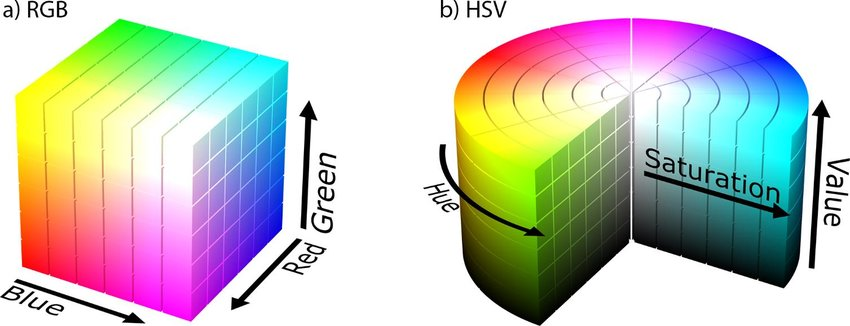
\includegraphics[width=\textwidth]{img/rgb_hsv.png}
    \caption{RGB and HSV colorspace comparison}
    \label{fig:rgb_hsv}
\end{figure}
The program utilizes color thresholding in combination with the images in the HSV colorspace to find the board in the scene and the grid which separates the sections. The thresholding values are stored in a JSON\footnote{JavaScript Object Notation} file, as they required experimentation to get right, and in the application settings file \textit{settings.json}, the color for the border and the grid is set. 

In the example from \autoref{fig:transformation}, the color of the border is \textit{red} and the color of the grid is \textit{black}, with both thresholded images seen in \autoref{fig:thresholding}.

\begin{figure}[h]%
    \centering
    \subfloat{\frame{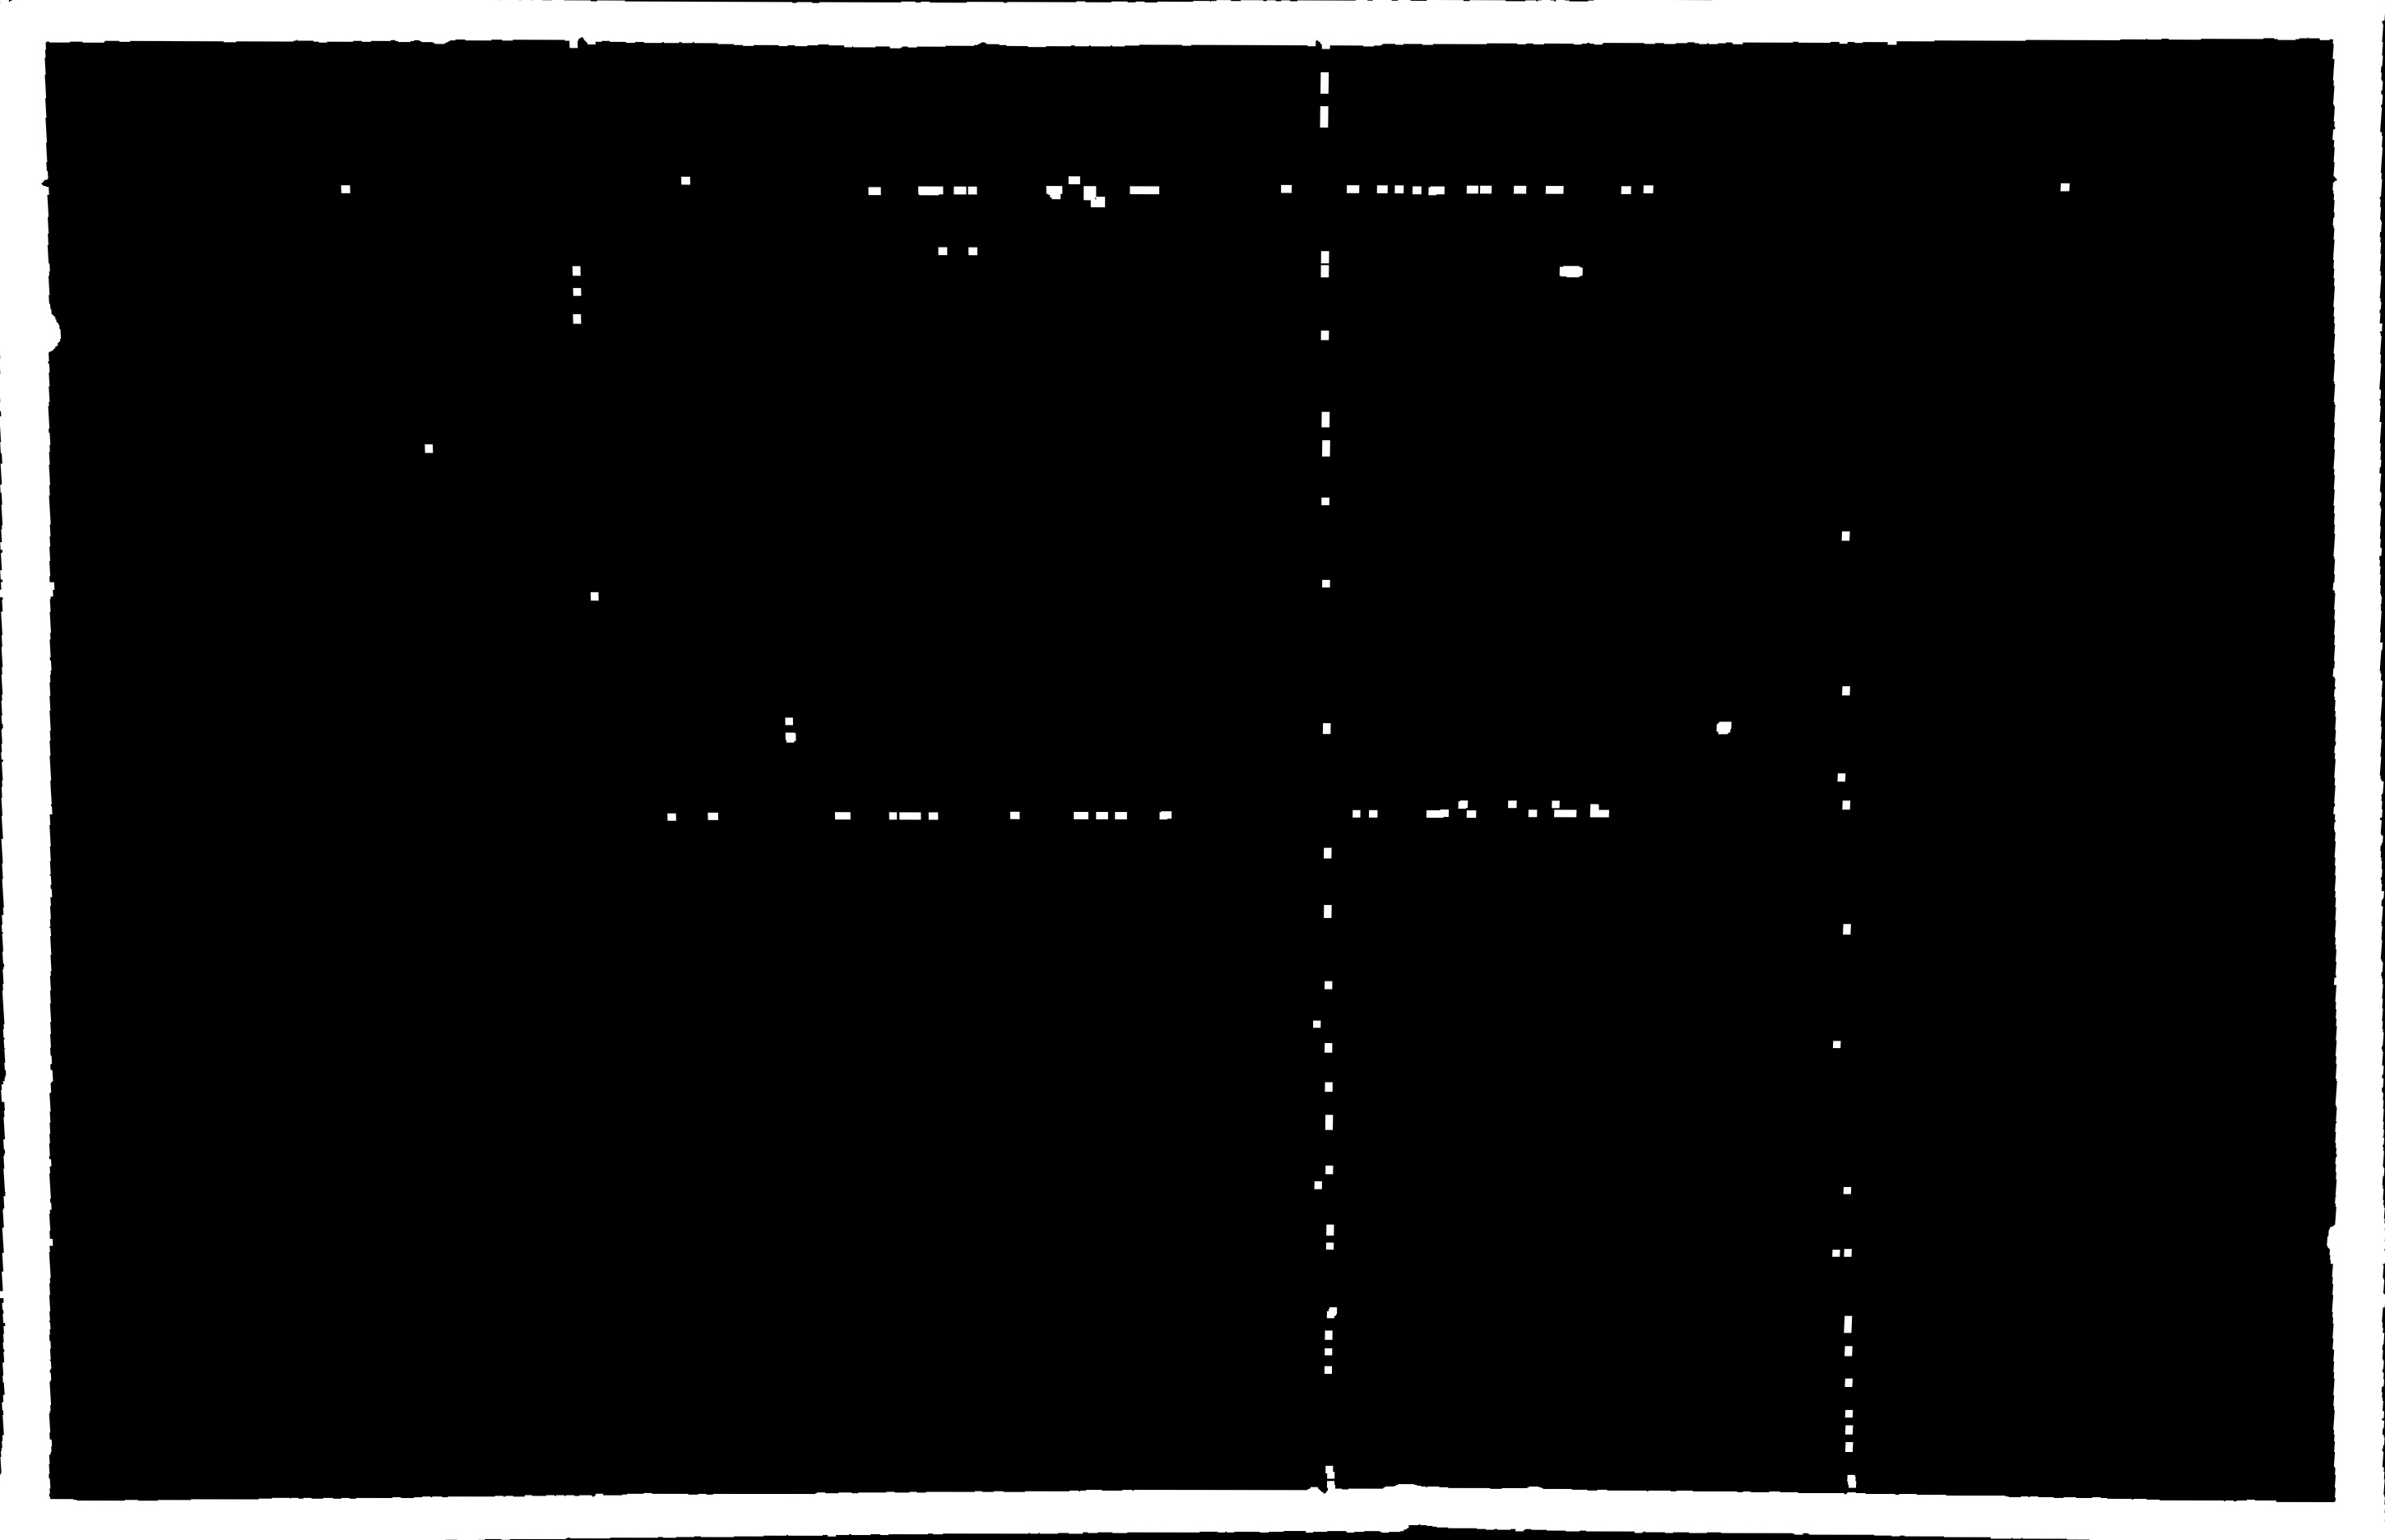
\includegraphics[width=6.6cm]{pipeline/warped_border.jpg}}}%
    \qquad
    \subfloat{\frame{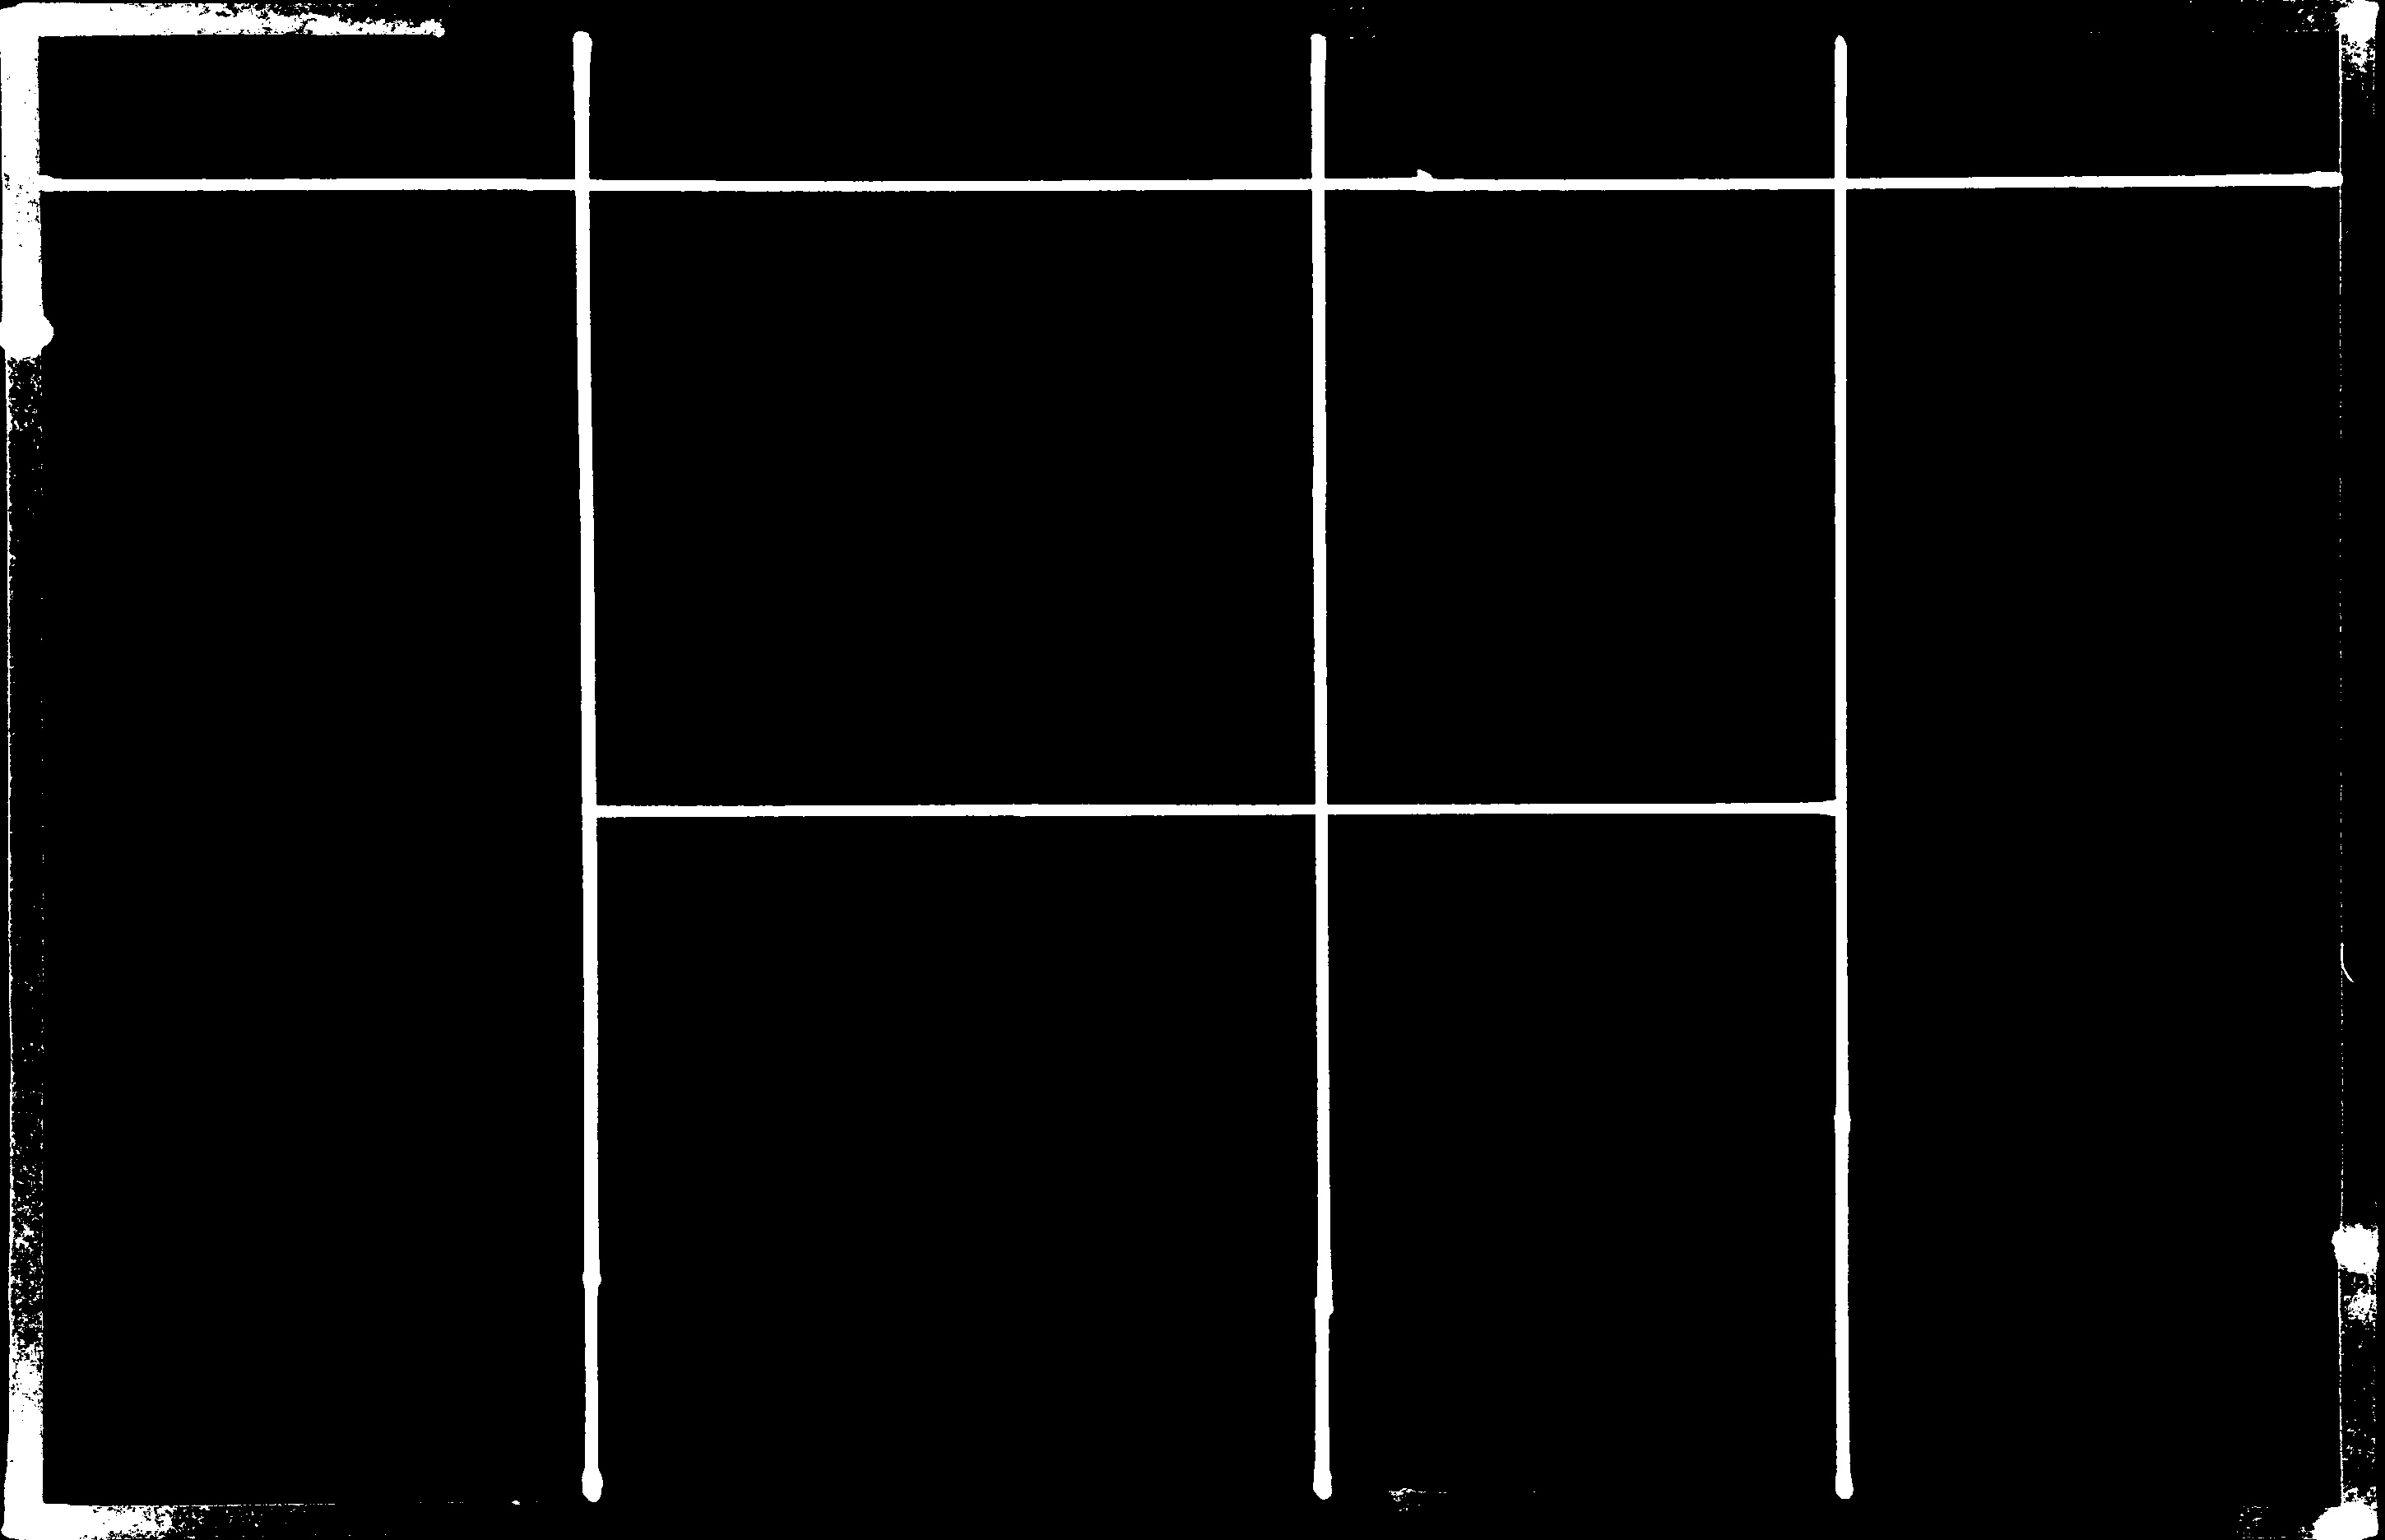
\includegraphics[width=6.6cm]{pipeline/sec_thresholded.jpg}}}%
    \caption{Thresholded border and grid of the transformed board}%
    \label{fig:thresholding}%
\end{figure}

\subsection{Board transformation}
Once the board itself is thresholded, an OpenCV function is used to classify the largest object in the thresholded image. If that object is a rectangle then the board is found and not obstructed, and the coordinates of the rectangle's corners recognized by the function in the thresholded image are used to transform\footnote{The operation of warping the image into a correct shape is also the one used in document scanning applications, which transform a document found in the image into a full screen scanned format\cite{doc_scan}.} the original image in such a way that it occupies the full scene, as seen in \autoref{fig:transformation}. The corner coordinates are used in the images after the initiation to transform the board.

\section{Finding the sections in the board}
\label{sec:finding_sec}
To detect how the tickets move from section to section, the program needs to detect what the areas of the sections are and to map those sections to sensible functions. Besides functions, the sections which contain tickets need to have a sensible name, and the program tackles all of those.

Below are all of the different functions that a section can have:
\begin{itemize}
    \item \textbf{None} - sections which serve no purpose at all, or were wrongfully classified as sections; these have no name
    \item \textbf{Limit} - sections which are used for placing the limit labels; these are mapped to ticket sections and denote the maximum permitted number of tickets that could be placed there at any moment; their name maps them to ticket sections automatically
    \item \textbf{Ticket} - these are sections for placing tickets; by default, they have a limit of 100, or they could have a limit preset from the \textit{Sections.json} or one set from a limit section
    \item \textbf{Final} - this section is the final one in the working pipeline; from here, the tickets are removed and marked as "done"
\end{itemize}

The images in \autoref{fig:thresholding} are combined to give the final image in \autoref{fig:sections_white}, that contains all of the sections in one image. Given that image, it is simple for OpenCV to detect all the blobs in the image, and assign them to sections. The sections are first assigned unique IDs based on their size, which can be used by a mapping algorithm to map to their respective names, functions, and limits.
\begin{figure}
    \centering
    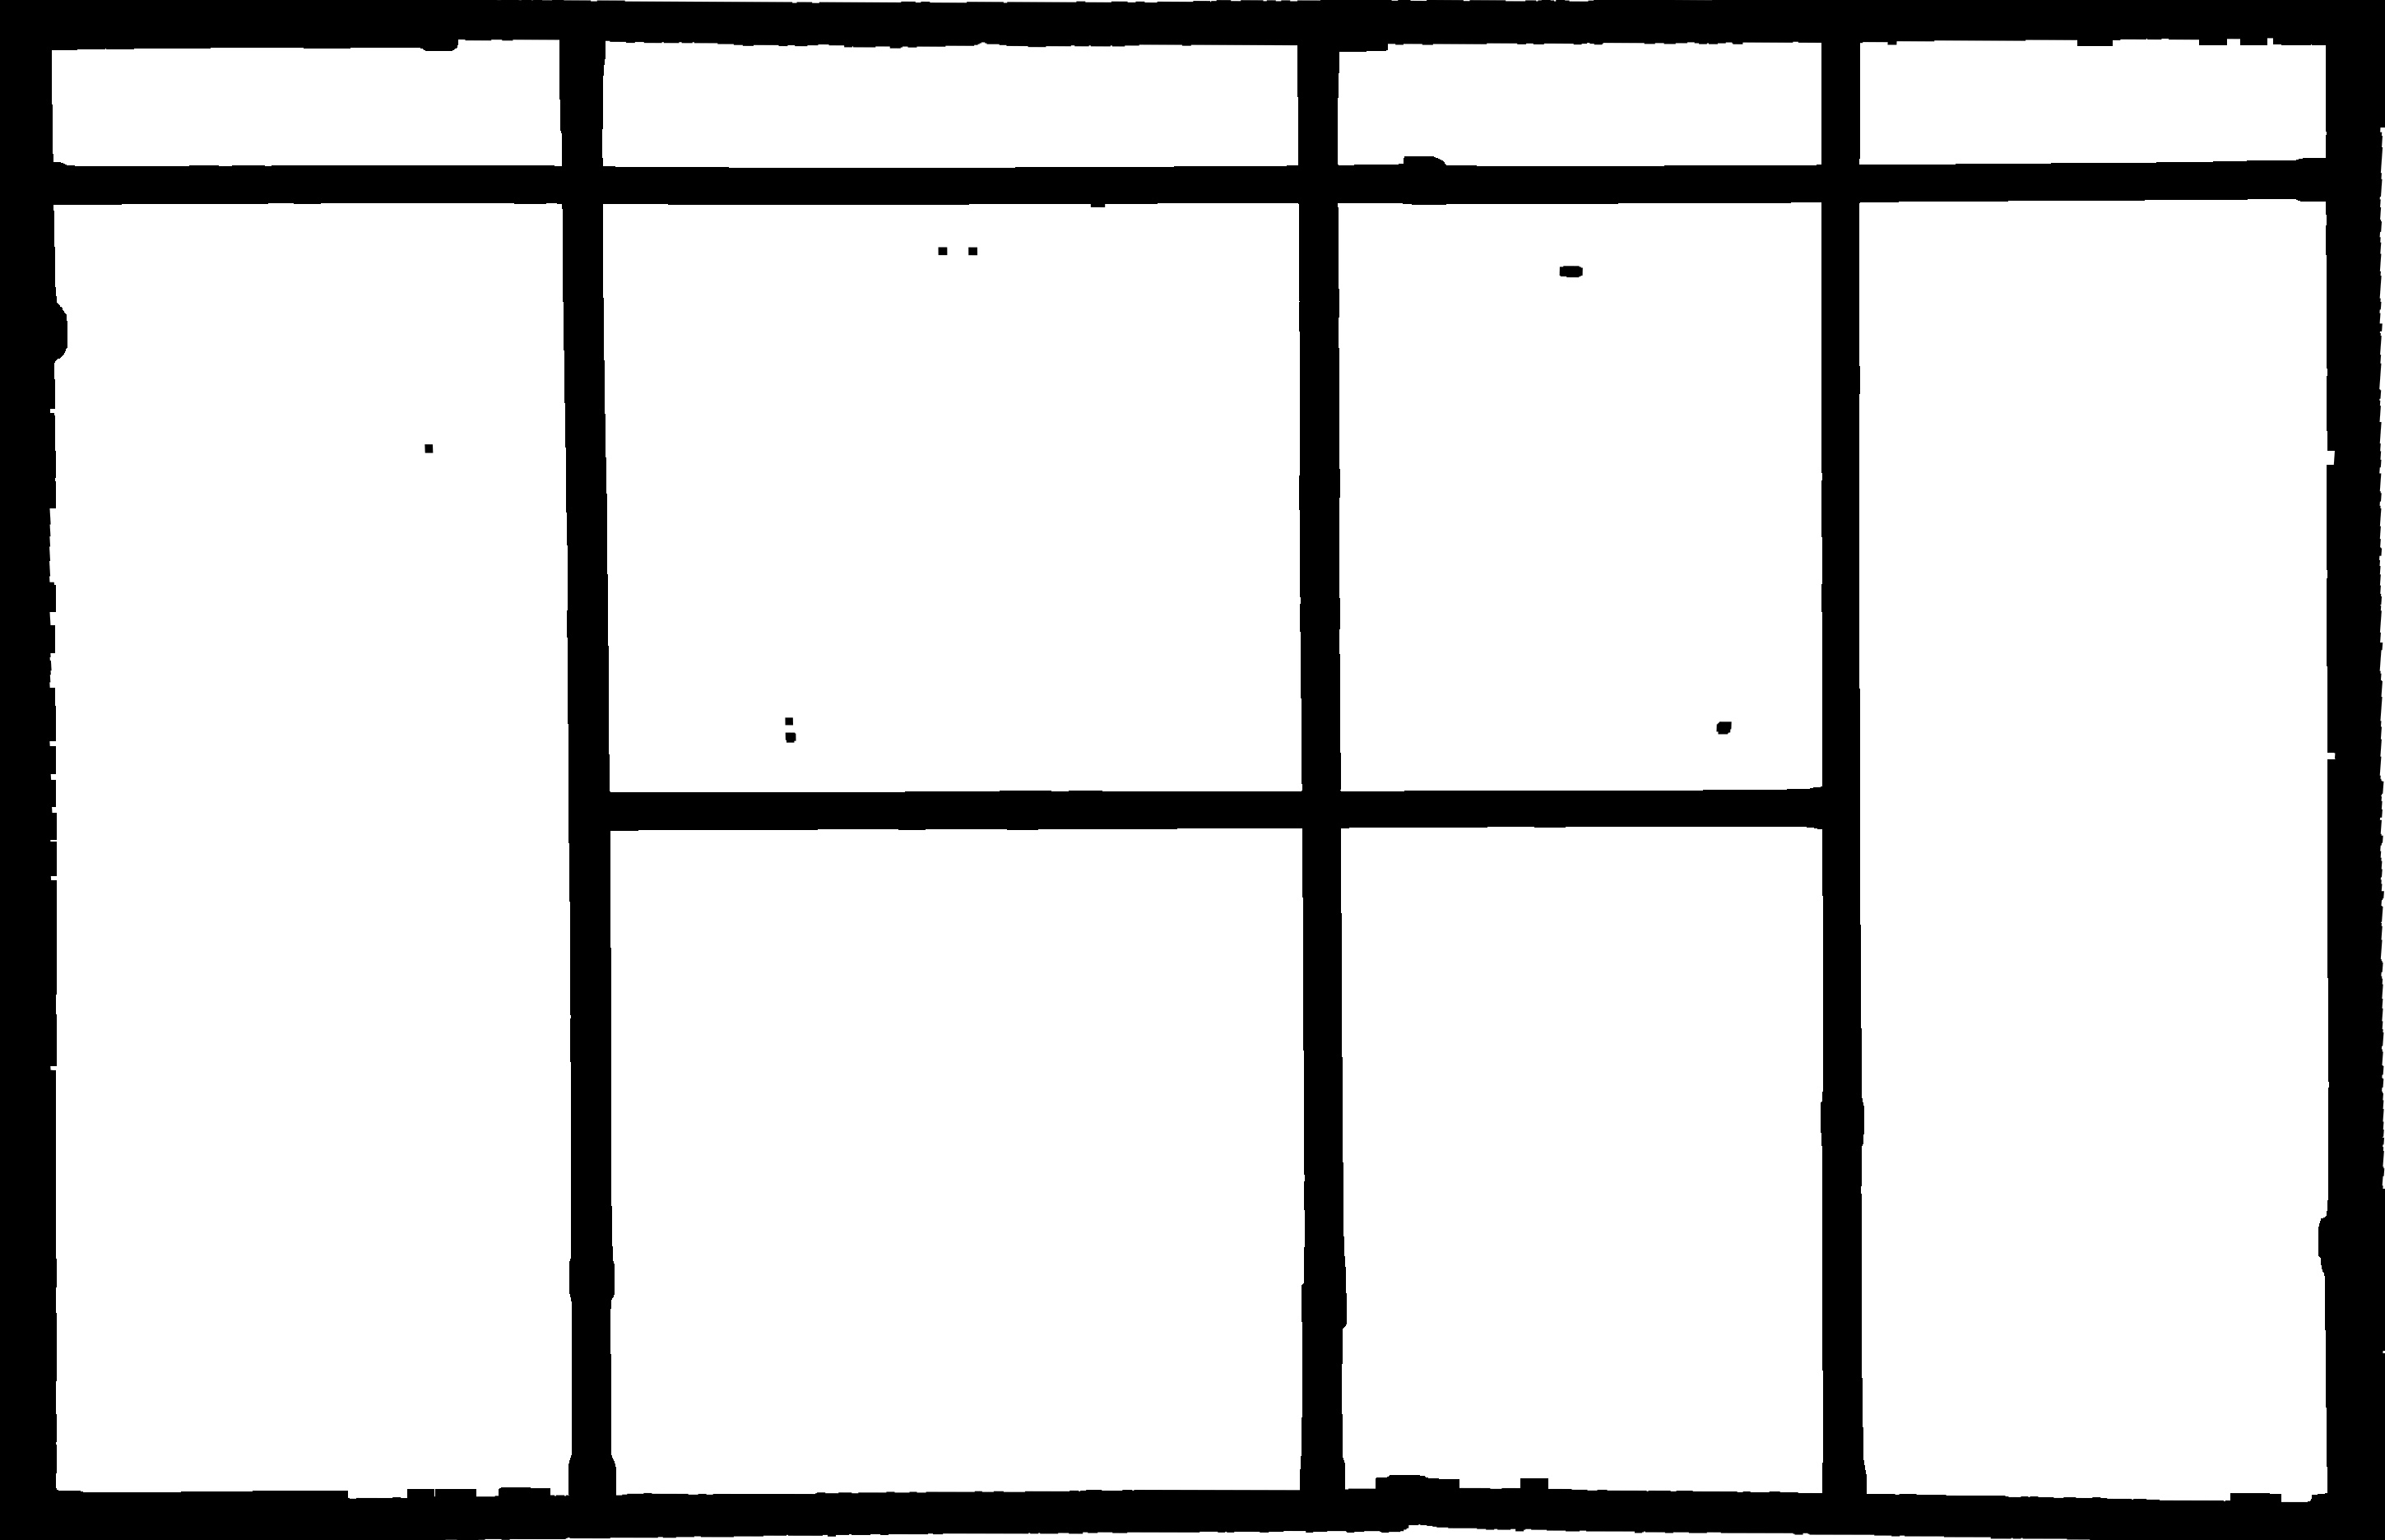
\includegraphics[width=\textwidth]{pipeline/sec_white_sections.jpg}
    \caption{All section masks in one image}
    \label{fig:sections_white}
\end{figure}

\chapter{Extracting Differences}
\section{Ticket movement detection}
To determine what the movements are, the program first needs a way to detect changes, which is done by HSV image differentiation on the \textbf{saturation} channel via the function in Listing \ref{lis:diff_mask}. Using that function, 3 different image masks are found:

\begin{enumerate}
    \item \textbf{curr\_prev\_diff} - the difference mask of the current and the previous photo
    \item \textbf{curr\_back\_diff} - the difference mask of the current and the background\footnote{The initial photo, used to set up the board. It contains no tickets, so it's treated as the background} photo
    \item \textbf{prev\_back\_diff} - the difference mask of the previous and the background photo
\end{enumerate}

These three may contain smaller regions of change, which can be noise and need to be filtered out. They are only an intermediate state, used to create the ticket masks:
\begin{enumerate}
    \item \textbf{added\_tickets\_mask} \ref{fig:added_removed} - contains tickets which were added to a section where they weren't previously - found by intersecting\footnote{The logical \textit{AND} operation performed on every pair of pixels from both images. White pixels are treated as 1, black pixels are treated as 0.} \textbf{curr\_prev\_diff} and \textbf{curr\_back\_diff}
    \item \textbf{removed\_tickets\_mask} \ref{fig:added_removed} - contains tickets which are no longer in a certain section - found by intersecting \textbf{curr\_prev\_diff} and \textbf{prev\_back\_diff}
\end{enumerate}

\begin{figure}[h]%
    \centering
    \subfloat{\frame{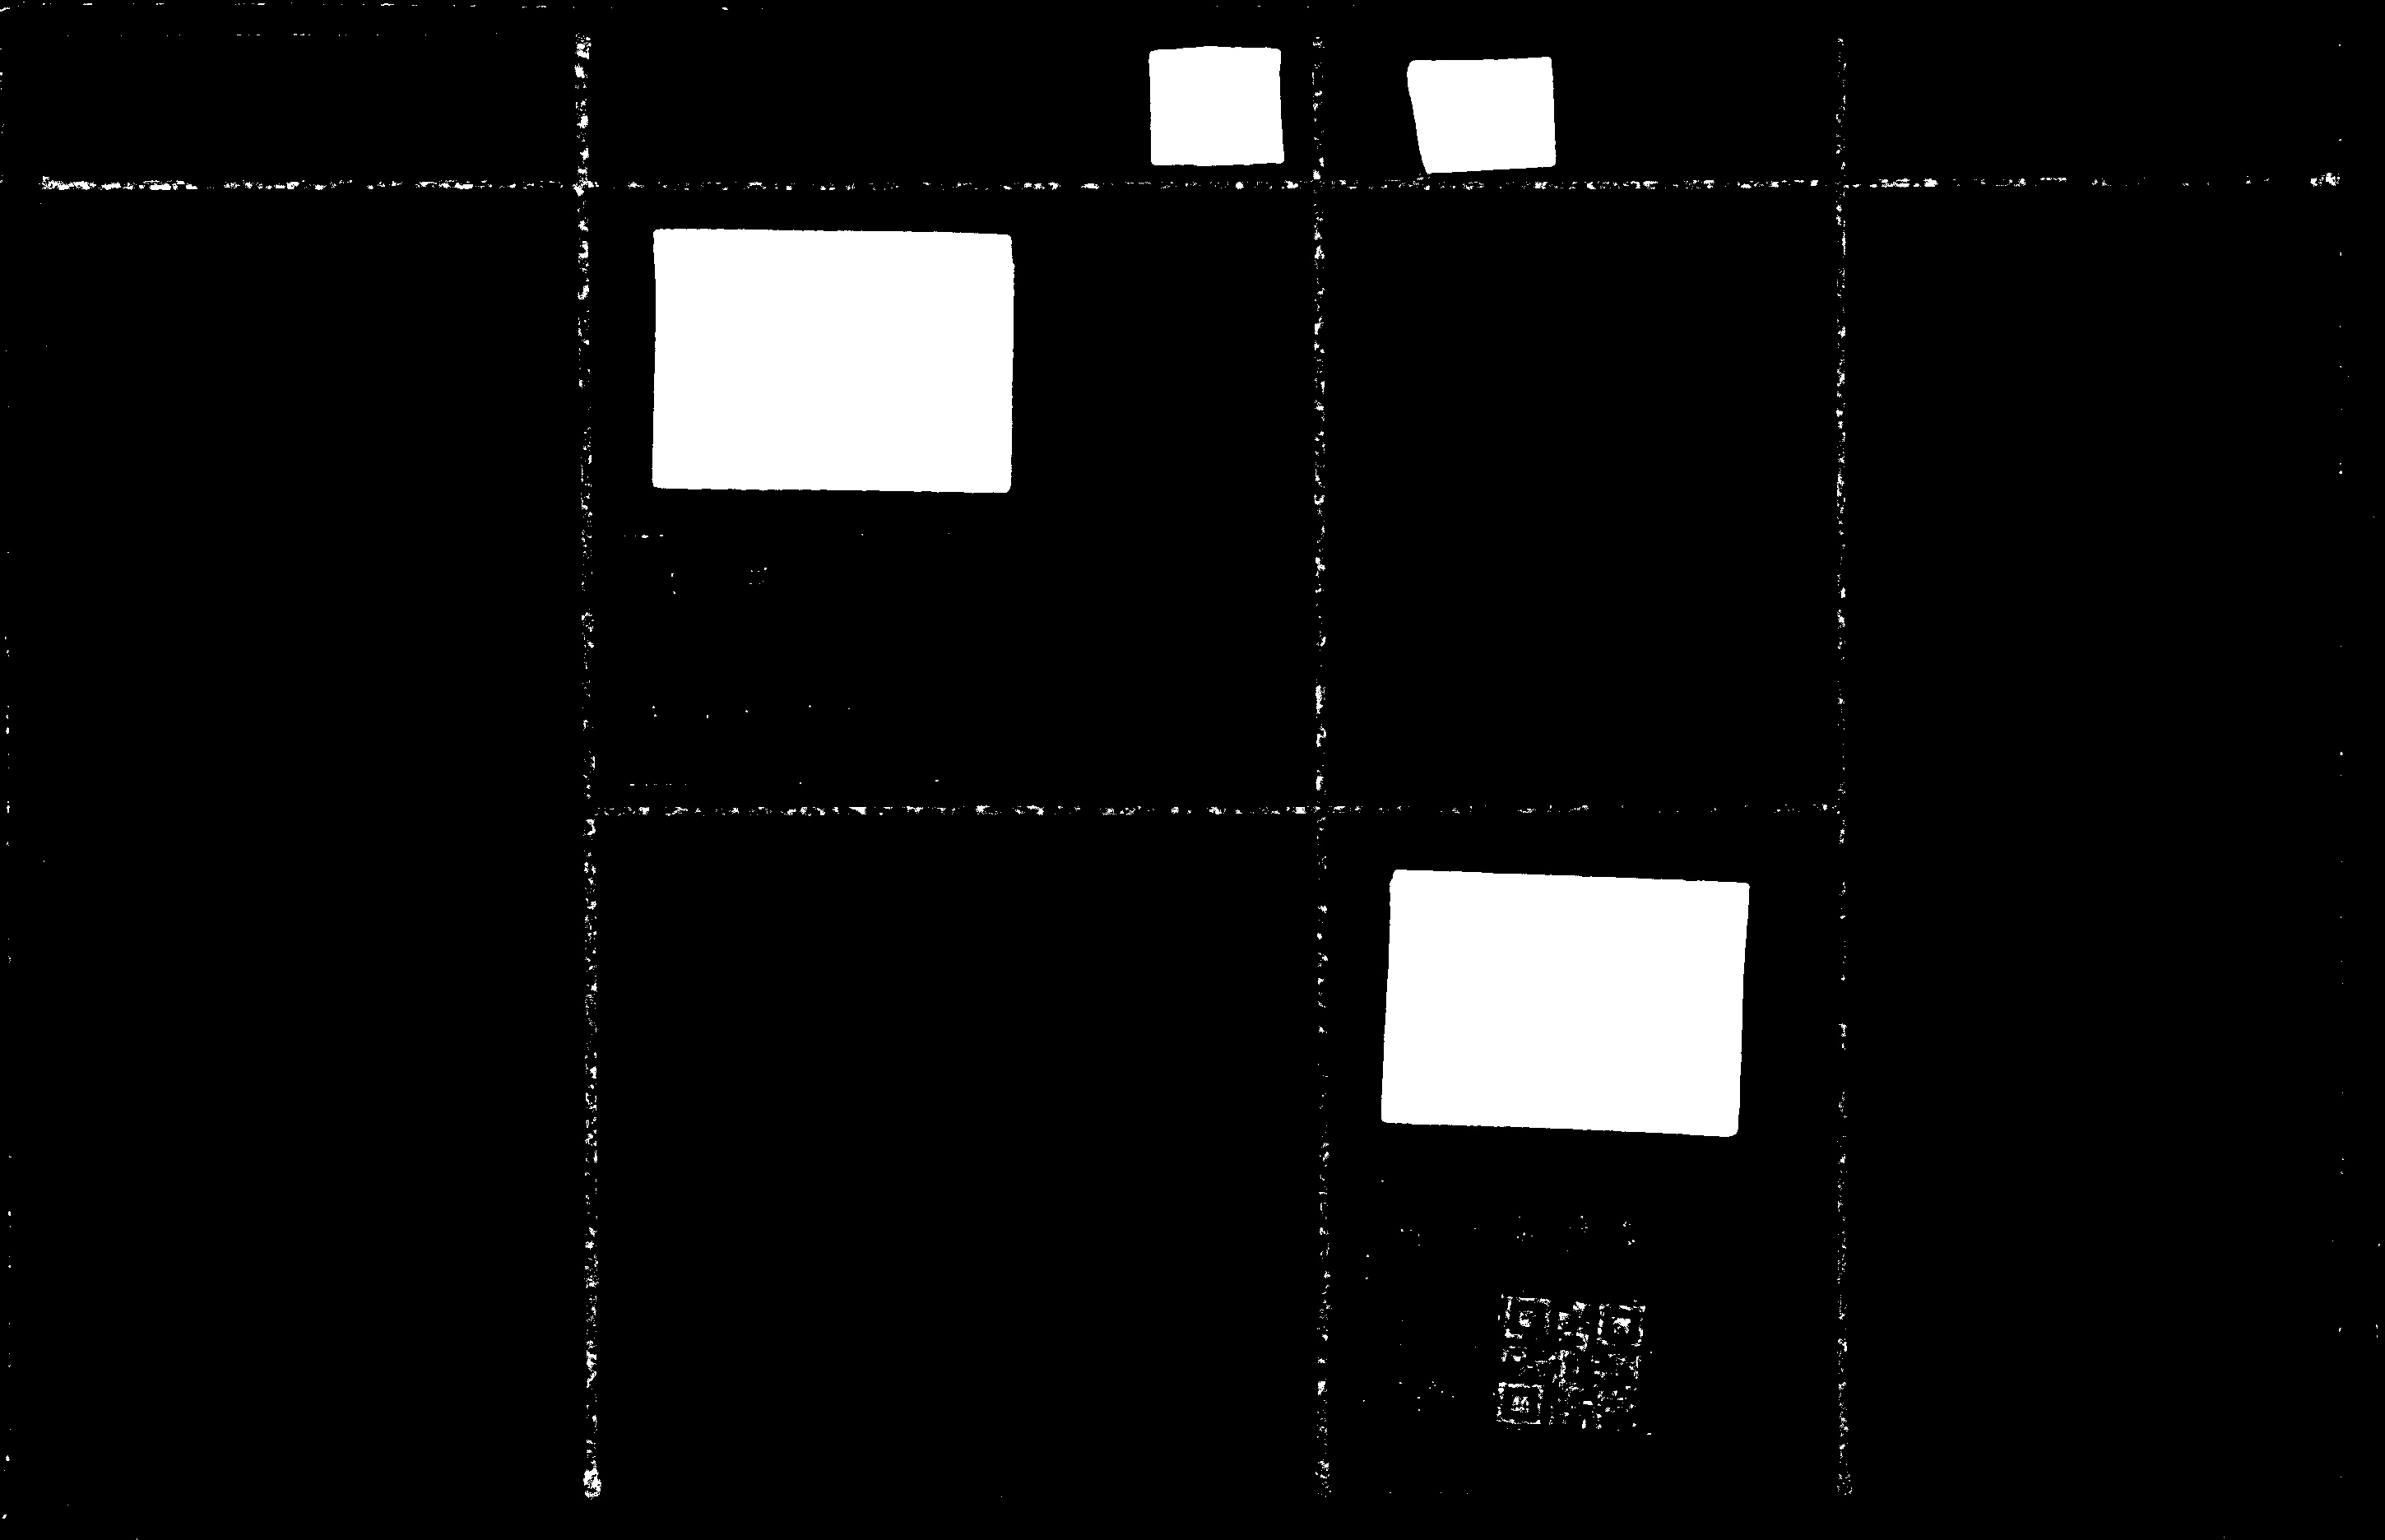
\includegraphics[width=6.6cm]{pipeline/added_ticket_mask.jpg}}}%
    \qquad
    \subfloat{\frame{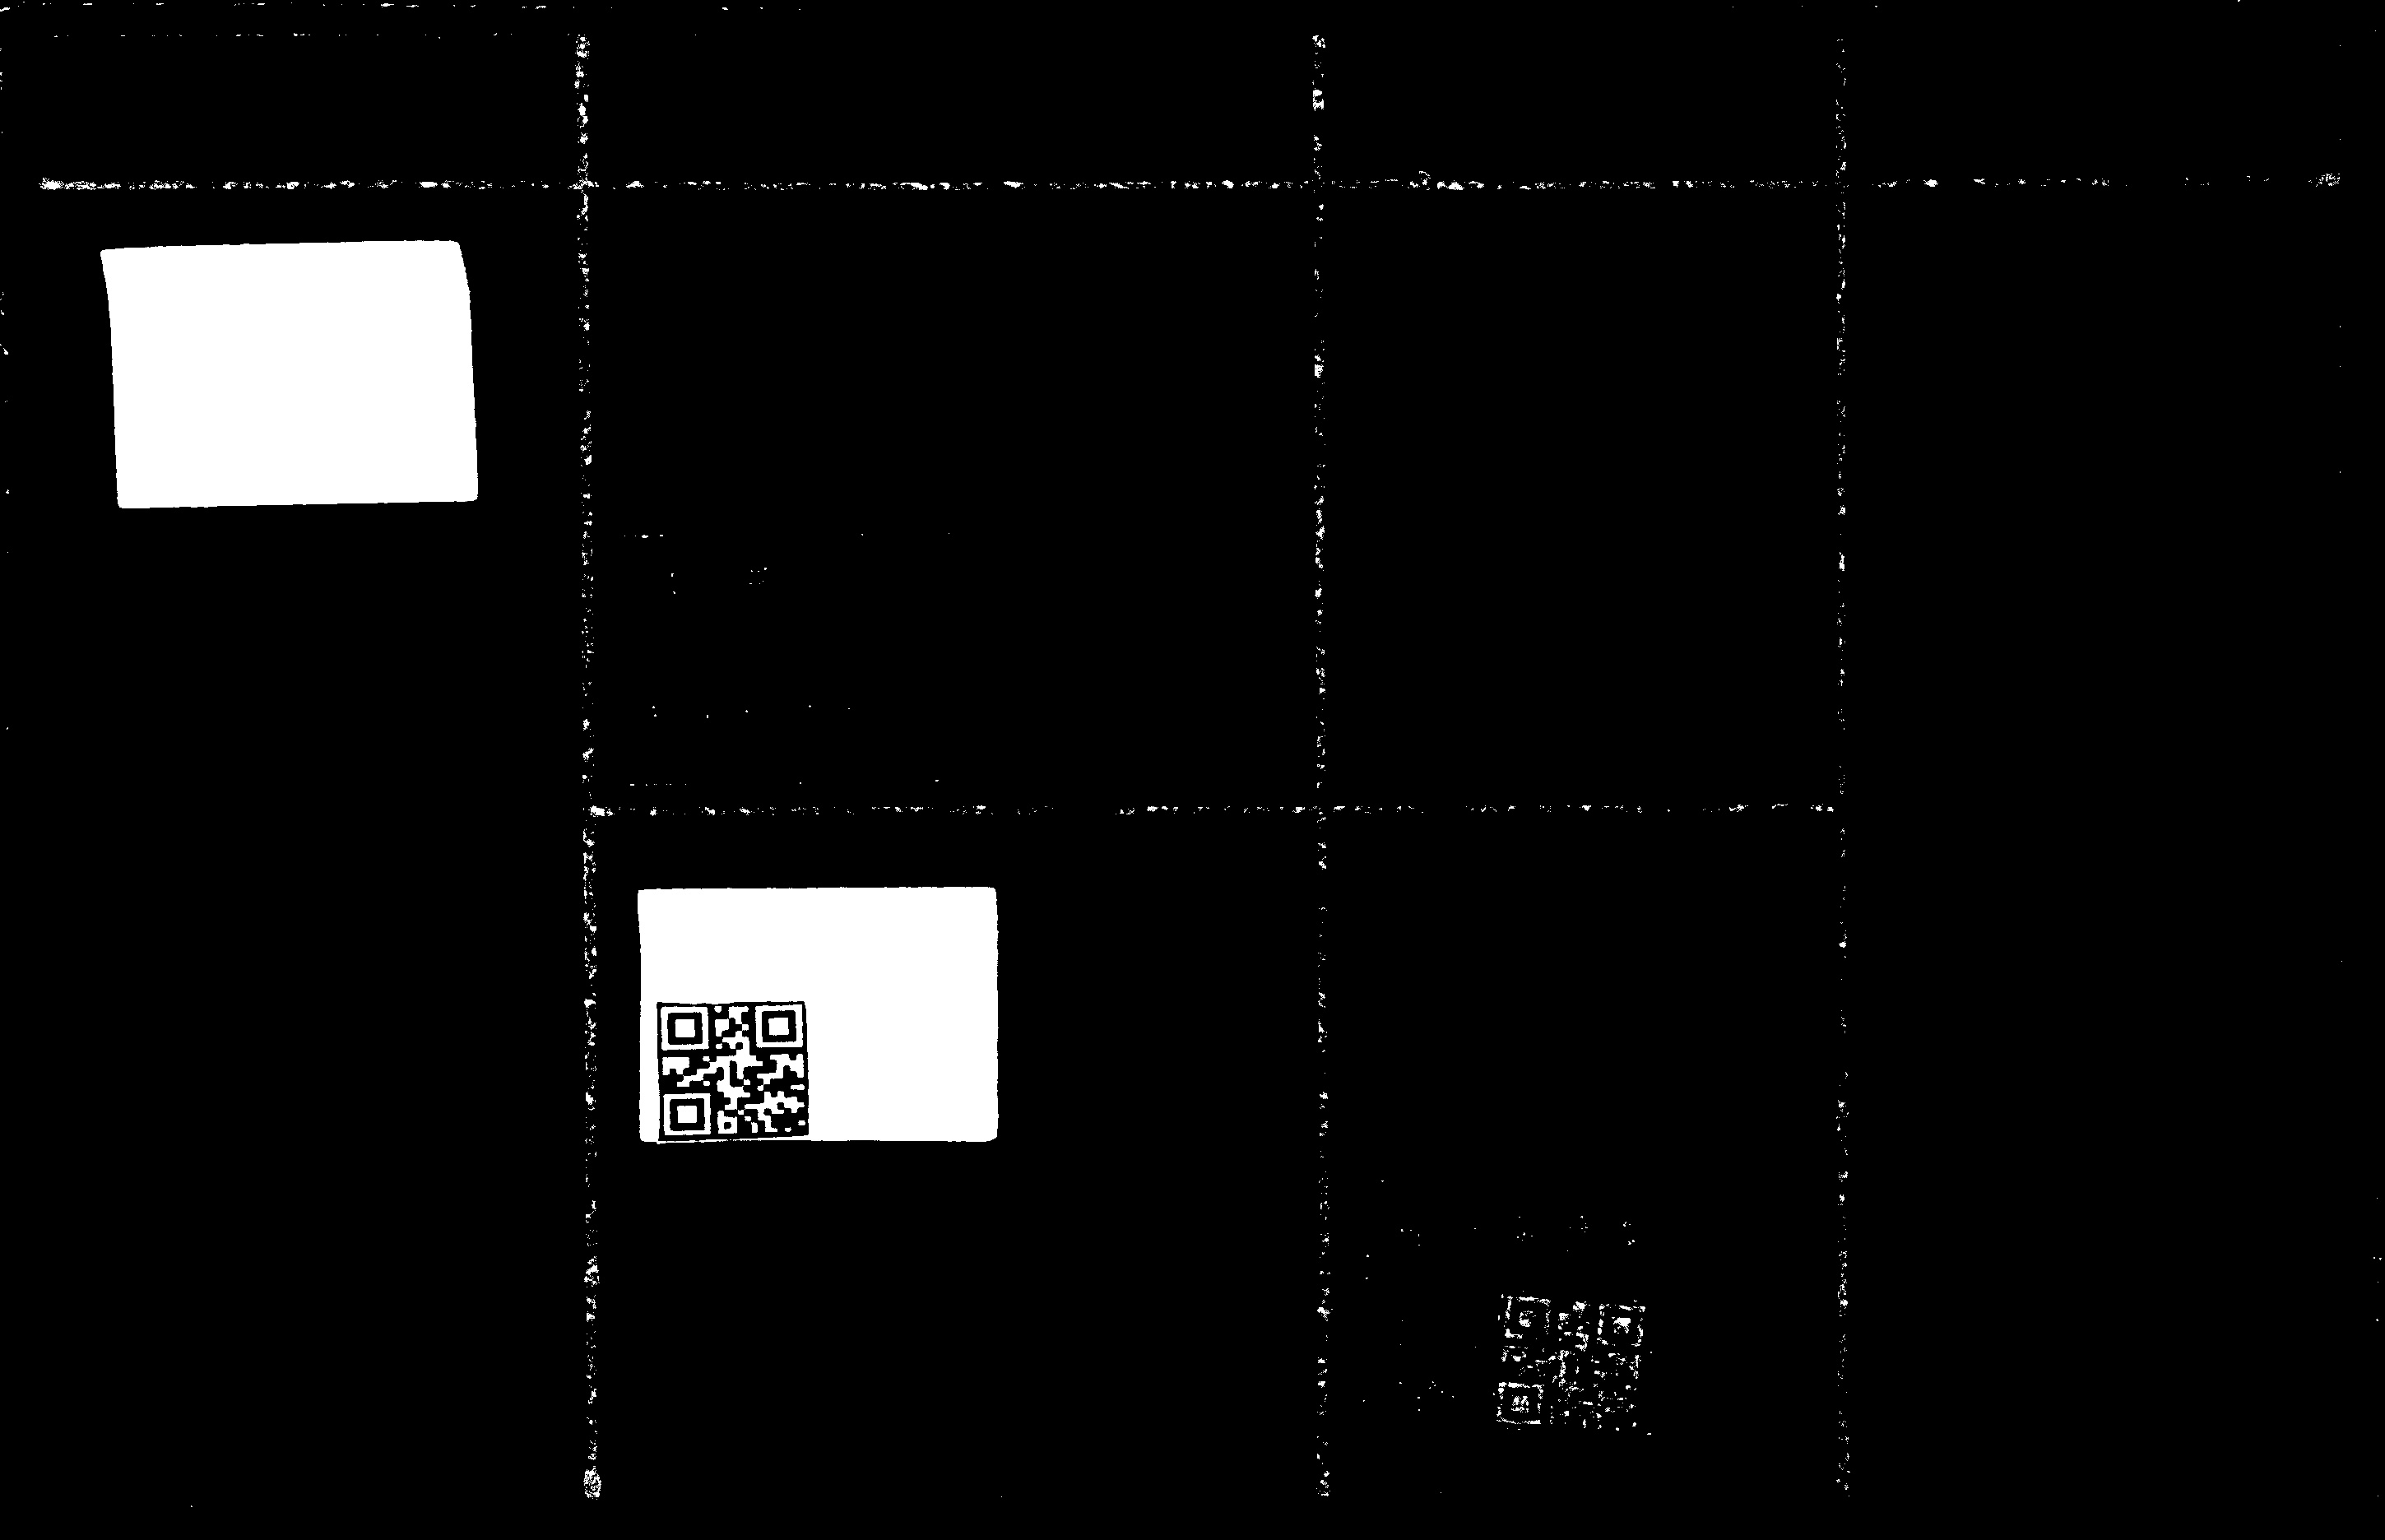
\includegraphics[width=6.6cm]{pipeline/removed_ticket_mask.jpg}}}%
    \caption{added\_tickets\_mask and removed\_tickets\_mask}%
    \label{fig:added_removed}%
\end{figure}

These two masks are the ones used to recognize the blobs\footnote{Regions that differ in properties, such as brightness or color, compared to surrounding regions.} that represent tickets. A ticket which has been removed from one section and moved to another is marked as \textit{moved} and has a line connecting the previous and the current region, as seen in \autoref{fig:visualized}.

\begin{scriptsize}
\python
\begin{lstlisting}[caption={Differencing function},captionpos=b]
# function which returns a mask of the differences between
# image1 and image2, which are in HSV format
def difference_mask(image1, image2, ticket_settings):
    # images are blurred by function normalize() and then
    # split into hue, saturation and value channels
    h1,s1,v1 = cv2.split(normalize(image1.copy()))
    h2,s2,v2 = cv2.split(normalize(image2.copy()))

    # creates an difference image which contains the pixel value 
    # differences of the saturation channel of the two images
    hsv_diff = cv2.absdiff(s1,s2)

    # create a mask from the difference image, colored white where  
    # the difference exceeds the threshold from the settings
    _, difference = cv2.threshold(hsv_diff, int(ticket_settings["difference_threshold"]), 255, cv2.THRESH_BINARY)
    
    return difference
\end{lstlisting}
\label{lis:diff_mask}
\end{scriptsize}
\section{Digit detection and classification}
There are numerous OCR\footnote{Optical Character Recognition} libraries, none of which can handle handwritten colored digits on an inconsistently colored background, which is why the project uses a unique approach for finding the digits on the tickets. Before arriving at the final method of digit detection, other methods were tested:

\begin{enumerate}
    \item \textbf{Sobel Edge Detection} - The method was successful in some lighting conditions, but as soon as the sharpness of the image was imperfect, it would fail to detect the digits on the ticket. It would also sometimes detect the edges of the tickets themselves as digits, which is incorrect.
    \item \textbf{Canny Edge Detection} - Similarly to Sobel, it was unsuccessful with images which didn't have perfect sharpness (i.e. contained noise) and failed to perform reliably.
    \item \textbf{Adaptive Thresholding} - Whilst it was reliable in finding the actual contours, thresholded digits themselves were not clear enough for the CNN\footnote{Convolutional Neural Network.} to classify.
    \begin{figure}[h]
        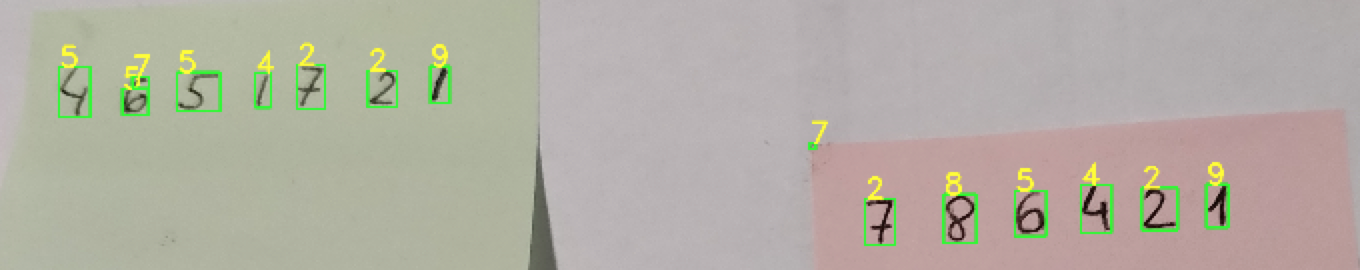
\includegraphics[width=0.93\textwidth,right]{img/adaptive_classification.png}
        \caption{Classification of contours found by adaptive thresholding}
    \end{figure}
    \item \textbf{Color Thresholding} - Unlike in other parts of the project, it failed to classify the digits completely. As the width of a pen stroke was roughly 5 pixels wide, the color of the tickets "bled" into the color of the digit, and the image file classified the digit as a darker shade of the ticket color that it was placed on \ref{fig:digits}.
    
    \begin{figure}%
        \centering
        \subfloat{{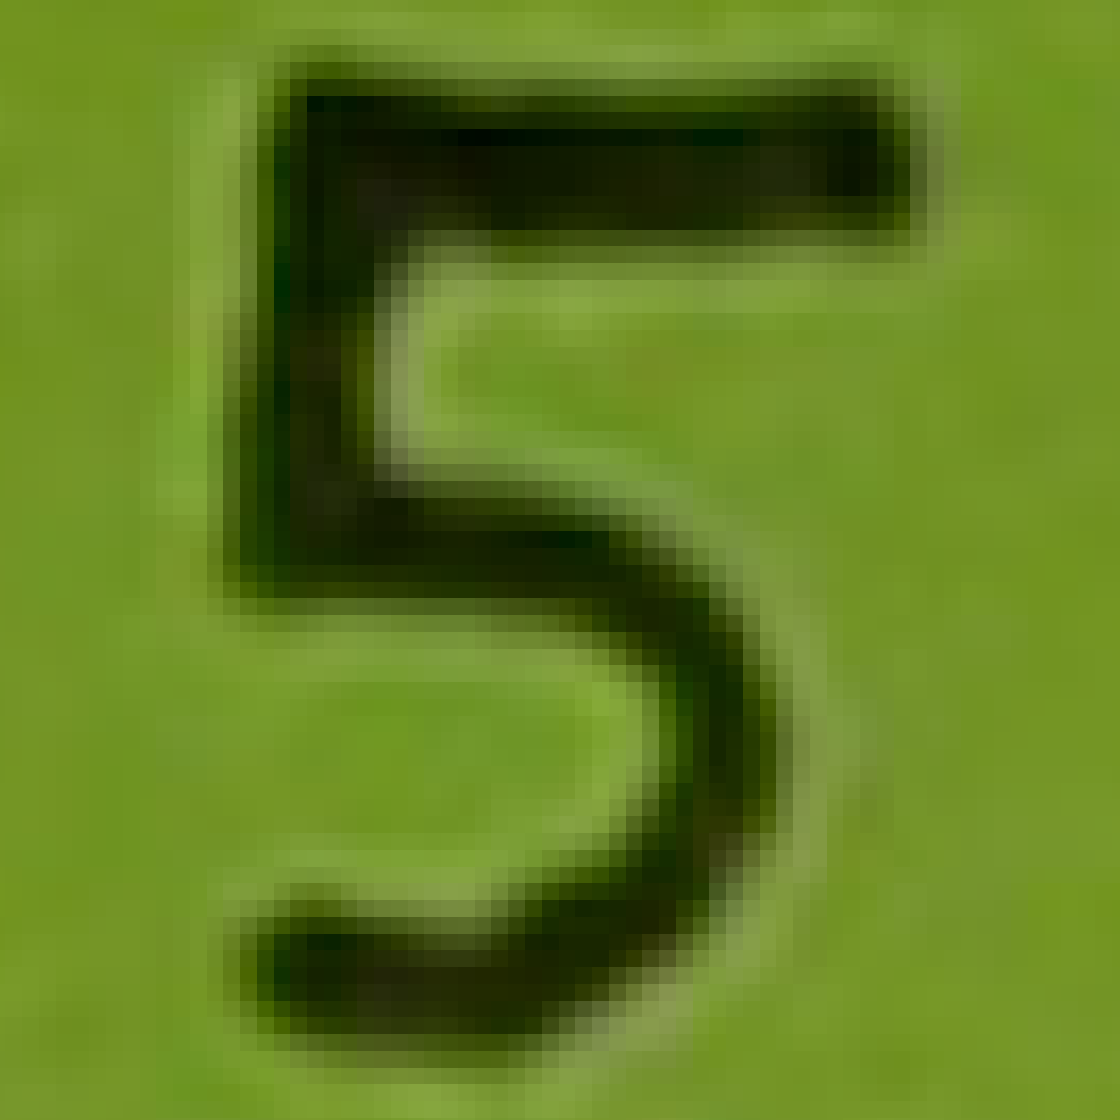
\includegraphics[width=3.2cm]{img/digit1.png} }}%
        \qquad
        \subfloat{{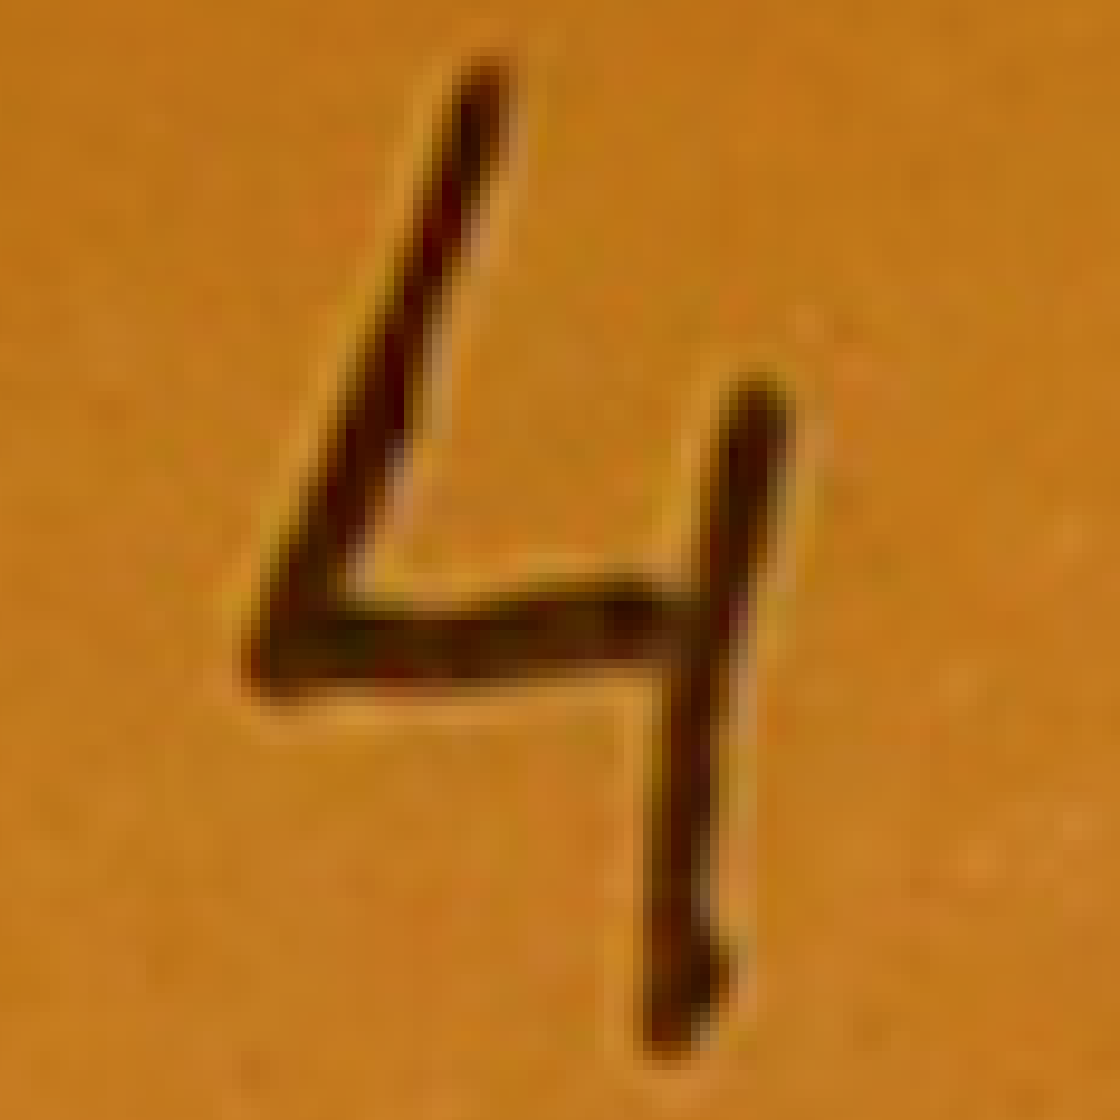
\includegraphics[width=3.2cm]{img/digit2.png} }}%
        \qquad
        \subfloat{{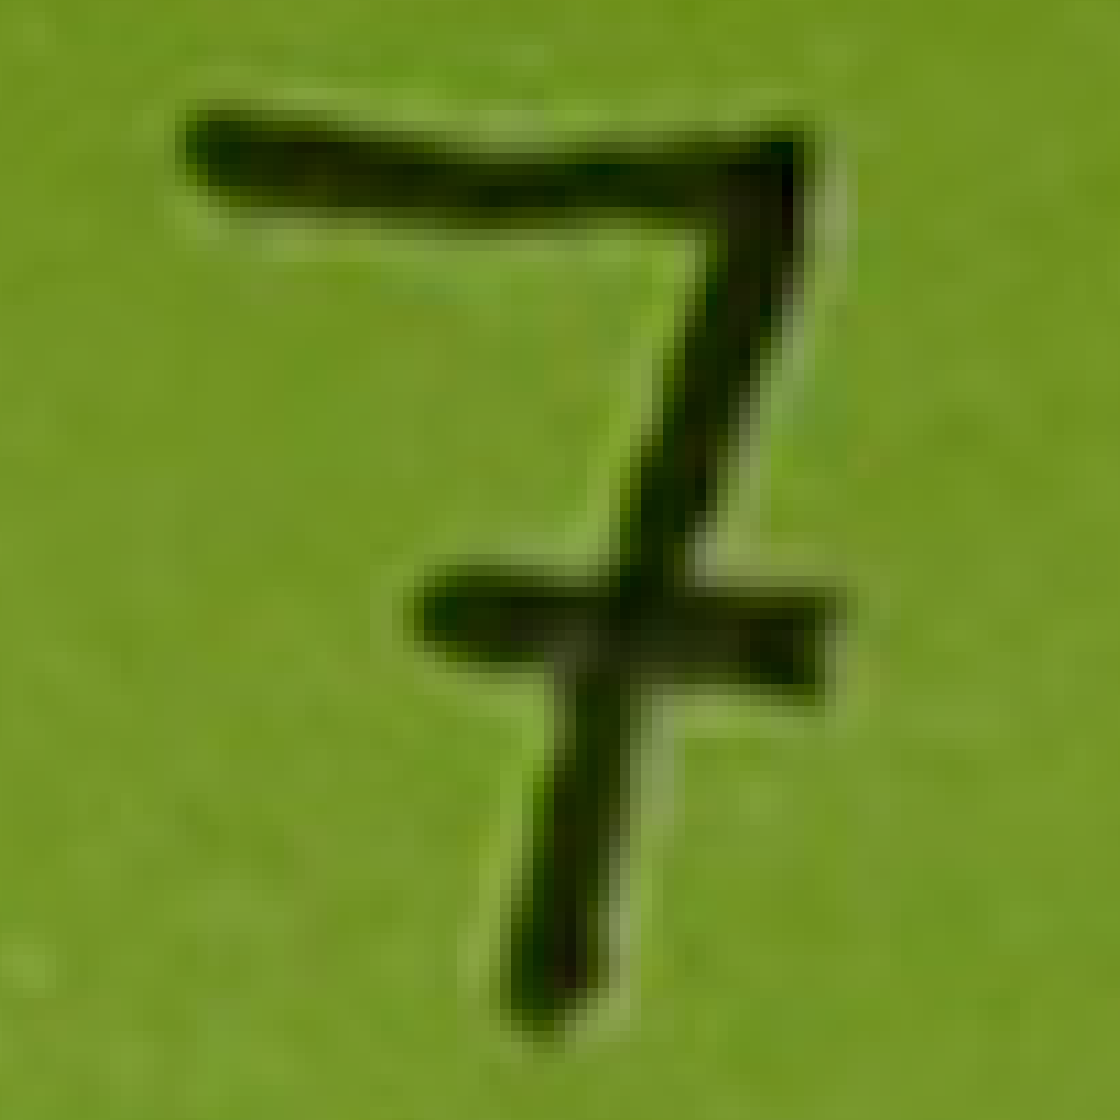
\includegraphics[width=3.2cm]{img/digit3.png} }}%
        \caption{Close up of digits being discolored by JPG compression}%
        \label{fig:digits}%
    \end{figure}
\end{enumerate}

All of the above methods failed, and the solution to the digit detection problem was \textbf{K-means clustering} \cite{kmeans}. It is a machine learning algorithm, which creates a number of groups of entries with similar qualities. In this case, these qualities are the RGB values of the individual pixels in a ticket region. In the application, the algorithm is instructed to detect 3 color groups from a region surrounding a ticket - the board (white), the ticket and the digit. The color of the digit will be the darkest, which is how we threshold it to detect the digit, an example of which is given in \autoref{fig:digit_thresholding}. After the thresholding step, the contours in the top portion (30\%) of the thresholded mask are passed to a CNN, which returns the recognized digit. Finally, the digits are concatenated to form the number on the ticket, which the application uses to identify it on the board.

\begin{figure}[h]%
    \centering
    \subfloat{\frame{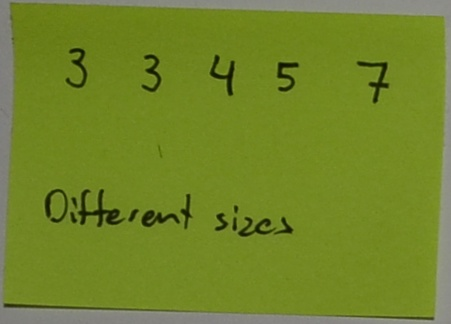
\includegraphics[width=6.6cm]{pipeline/digit_original.jpg}}}%
    \qquad
    \subfloat{\frame{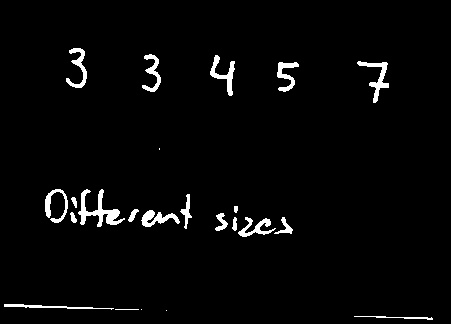
\includegraphics[width=6.6cm]{pipeline/digit_mask.jpg}}}%
    \caption{Ticket area before and after clustering and thresholding}%
    \label{fig:digit_thresholding}%
\end{figure}

\section{Tag detection}
The tags themselves are detected using the \textbf{pyzbar} library, available to install through PIP\footnote{\url{https://pypi.org/project/pip/}}. It provides functions for detecting QR codes and barcodes, from images that are loaded via OpenCV. From the supplied image, the library returns the content\footnote{The string that the QR code contains. The string itself is the name of the assignee for the ticket.} and the coordinates of the QR codes. The coordinates are used for creating the assignee masks \ref{fig:assignee_masks}, which denote the area that individual tags occupy in the photo. By looping through the ticket masks, an algorithm assigns each ticket to the assignee found in the tag that's found in its area.



\begin{figure}[h]%
    \centering
    \subfloat{\frame{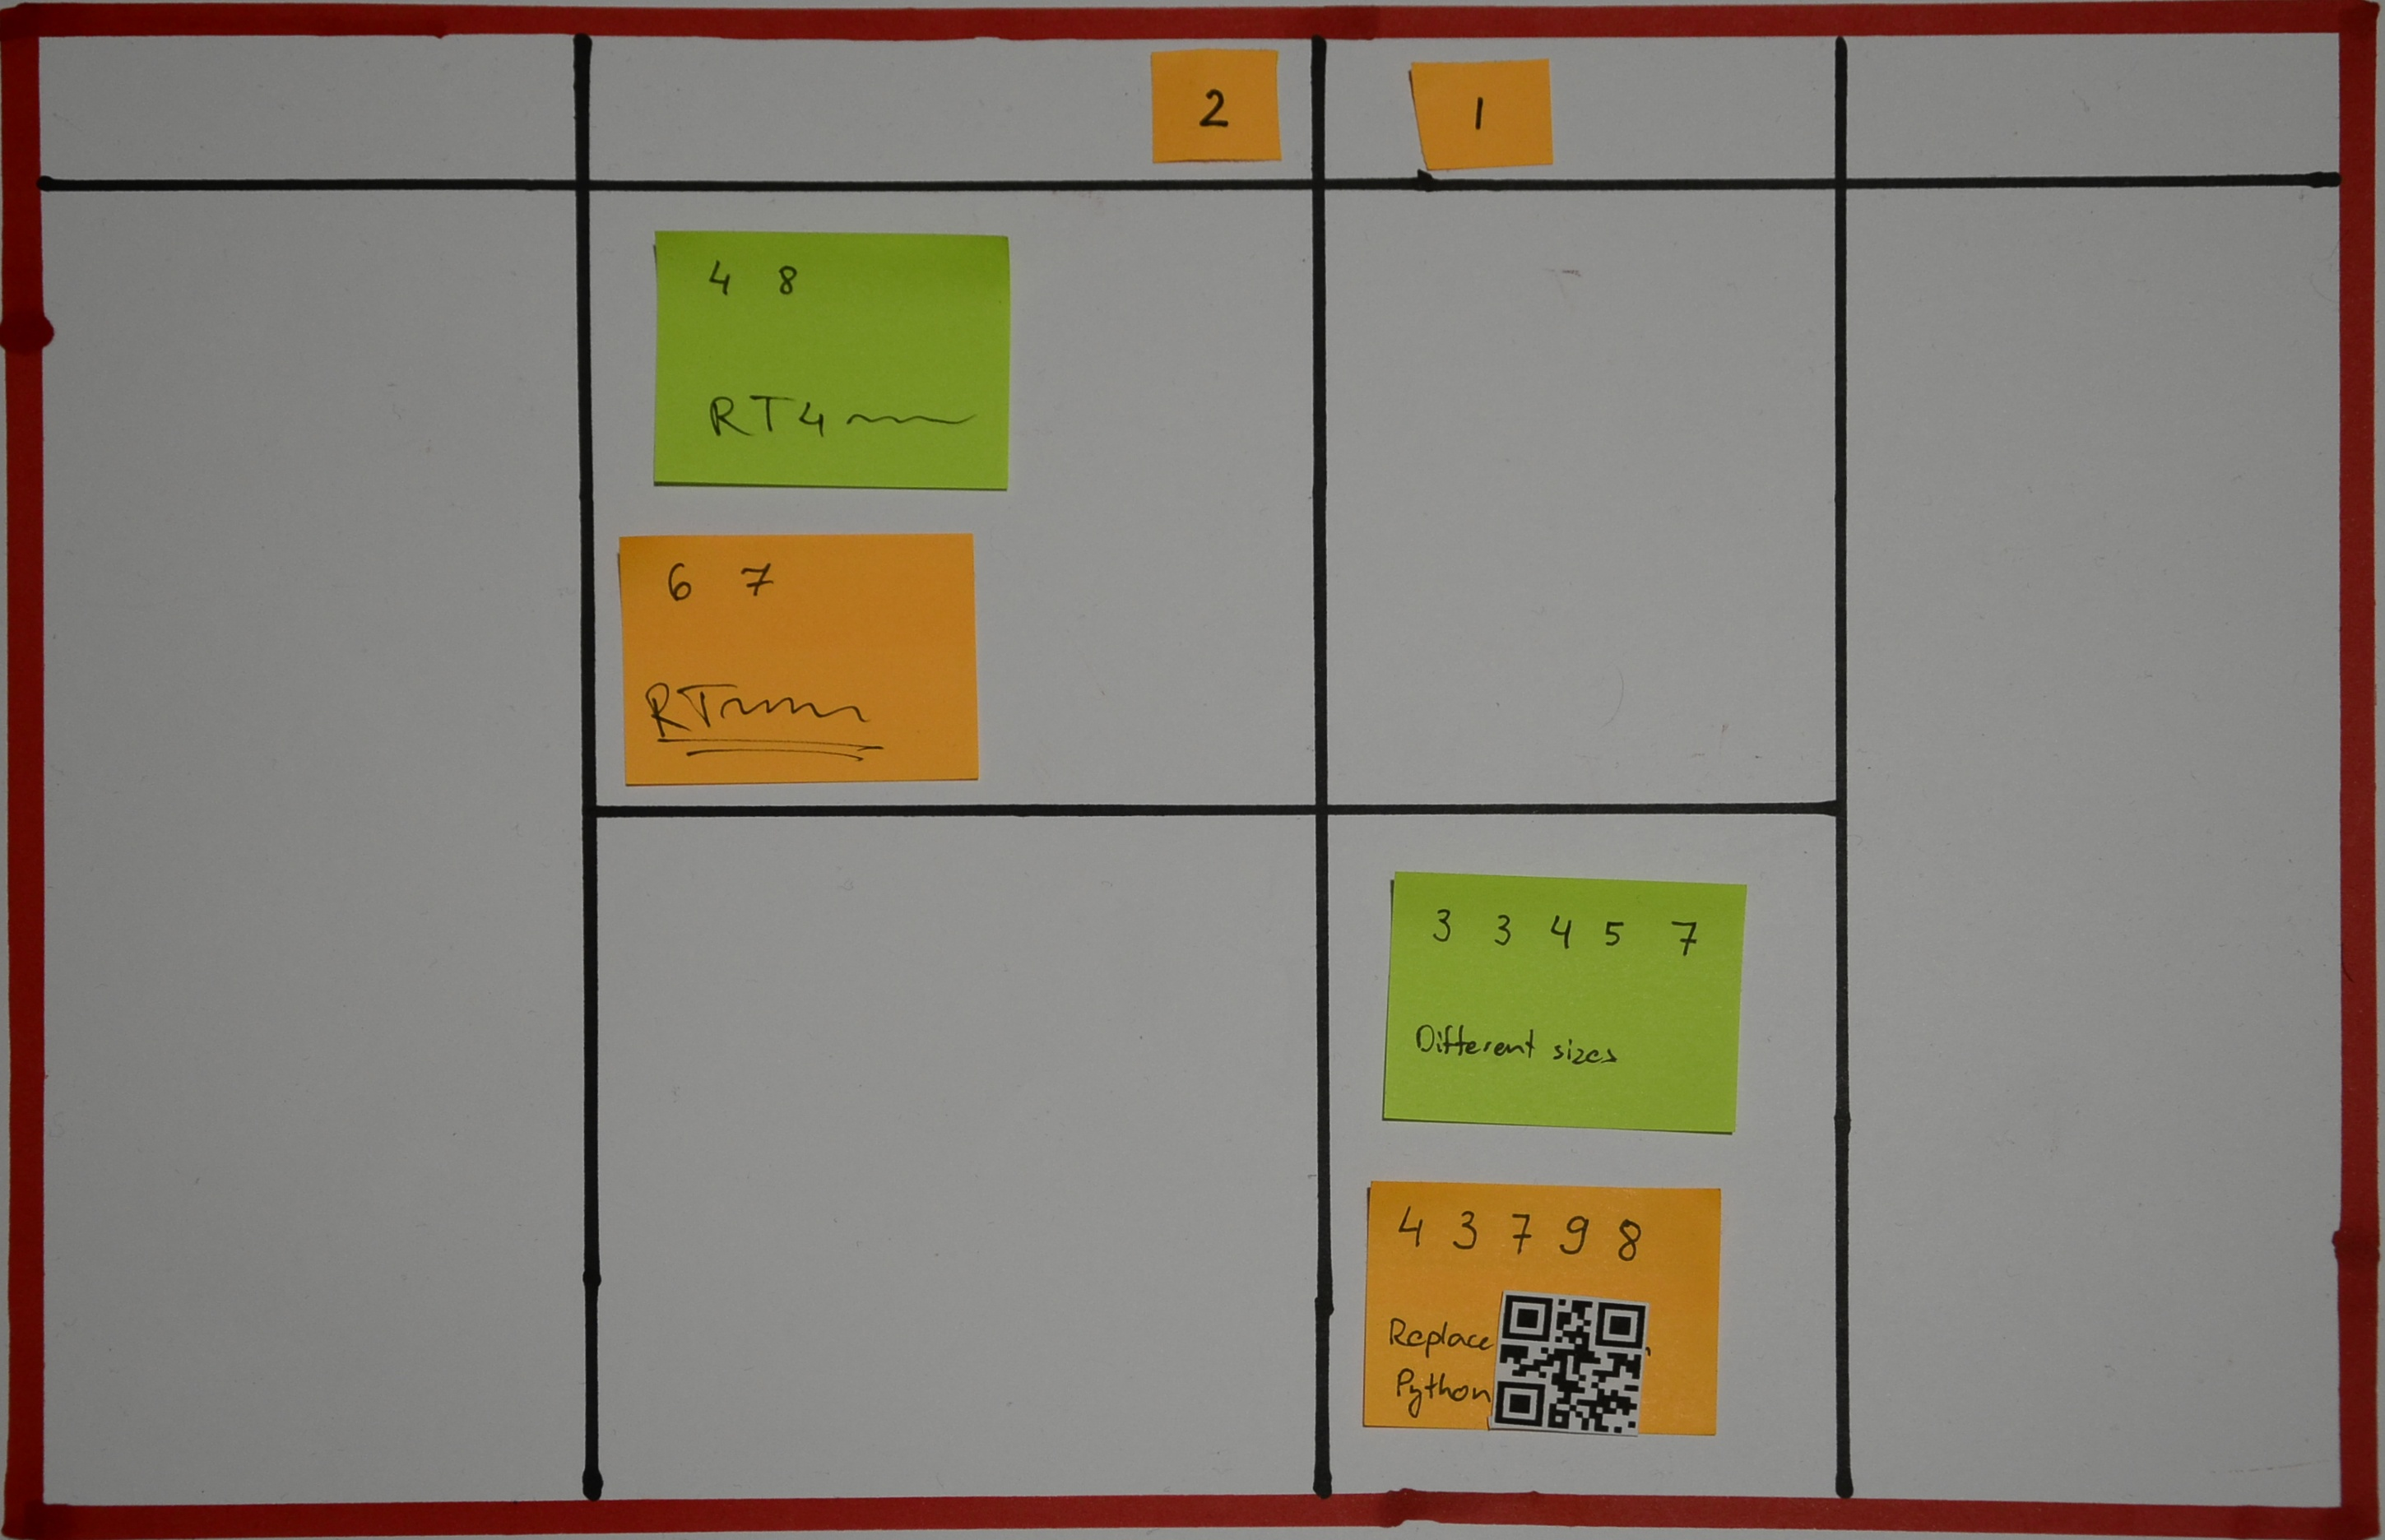
\includegraphics[width=6.6cm]{pipeline/tic_assignee_image1.jpg}}}%
    \qquad
    \subfloat{\frame{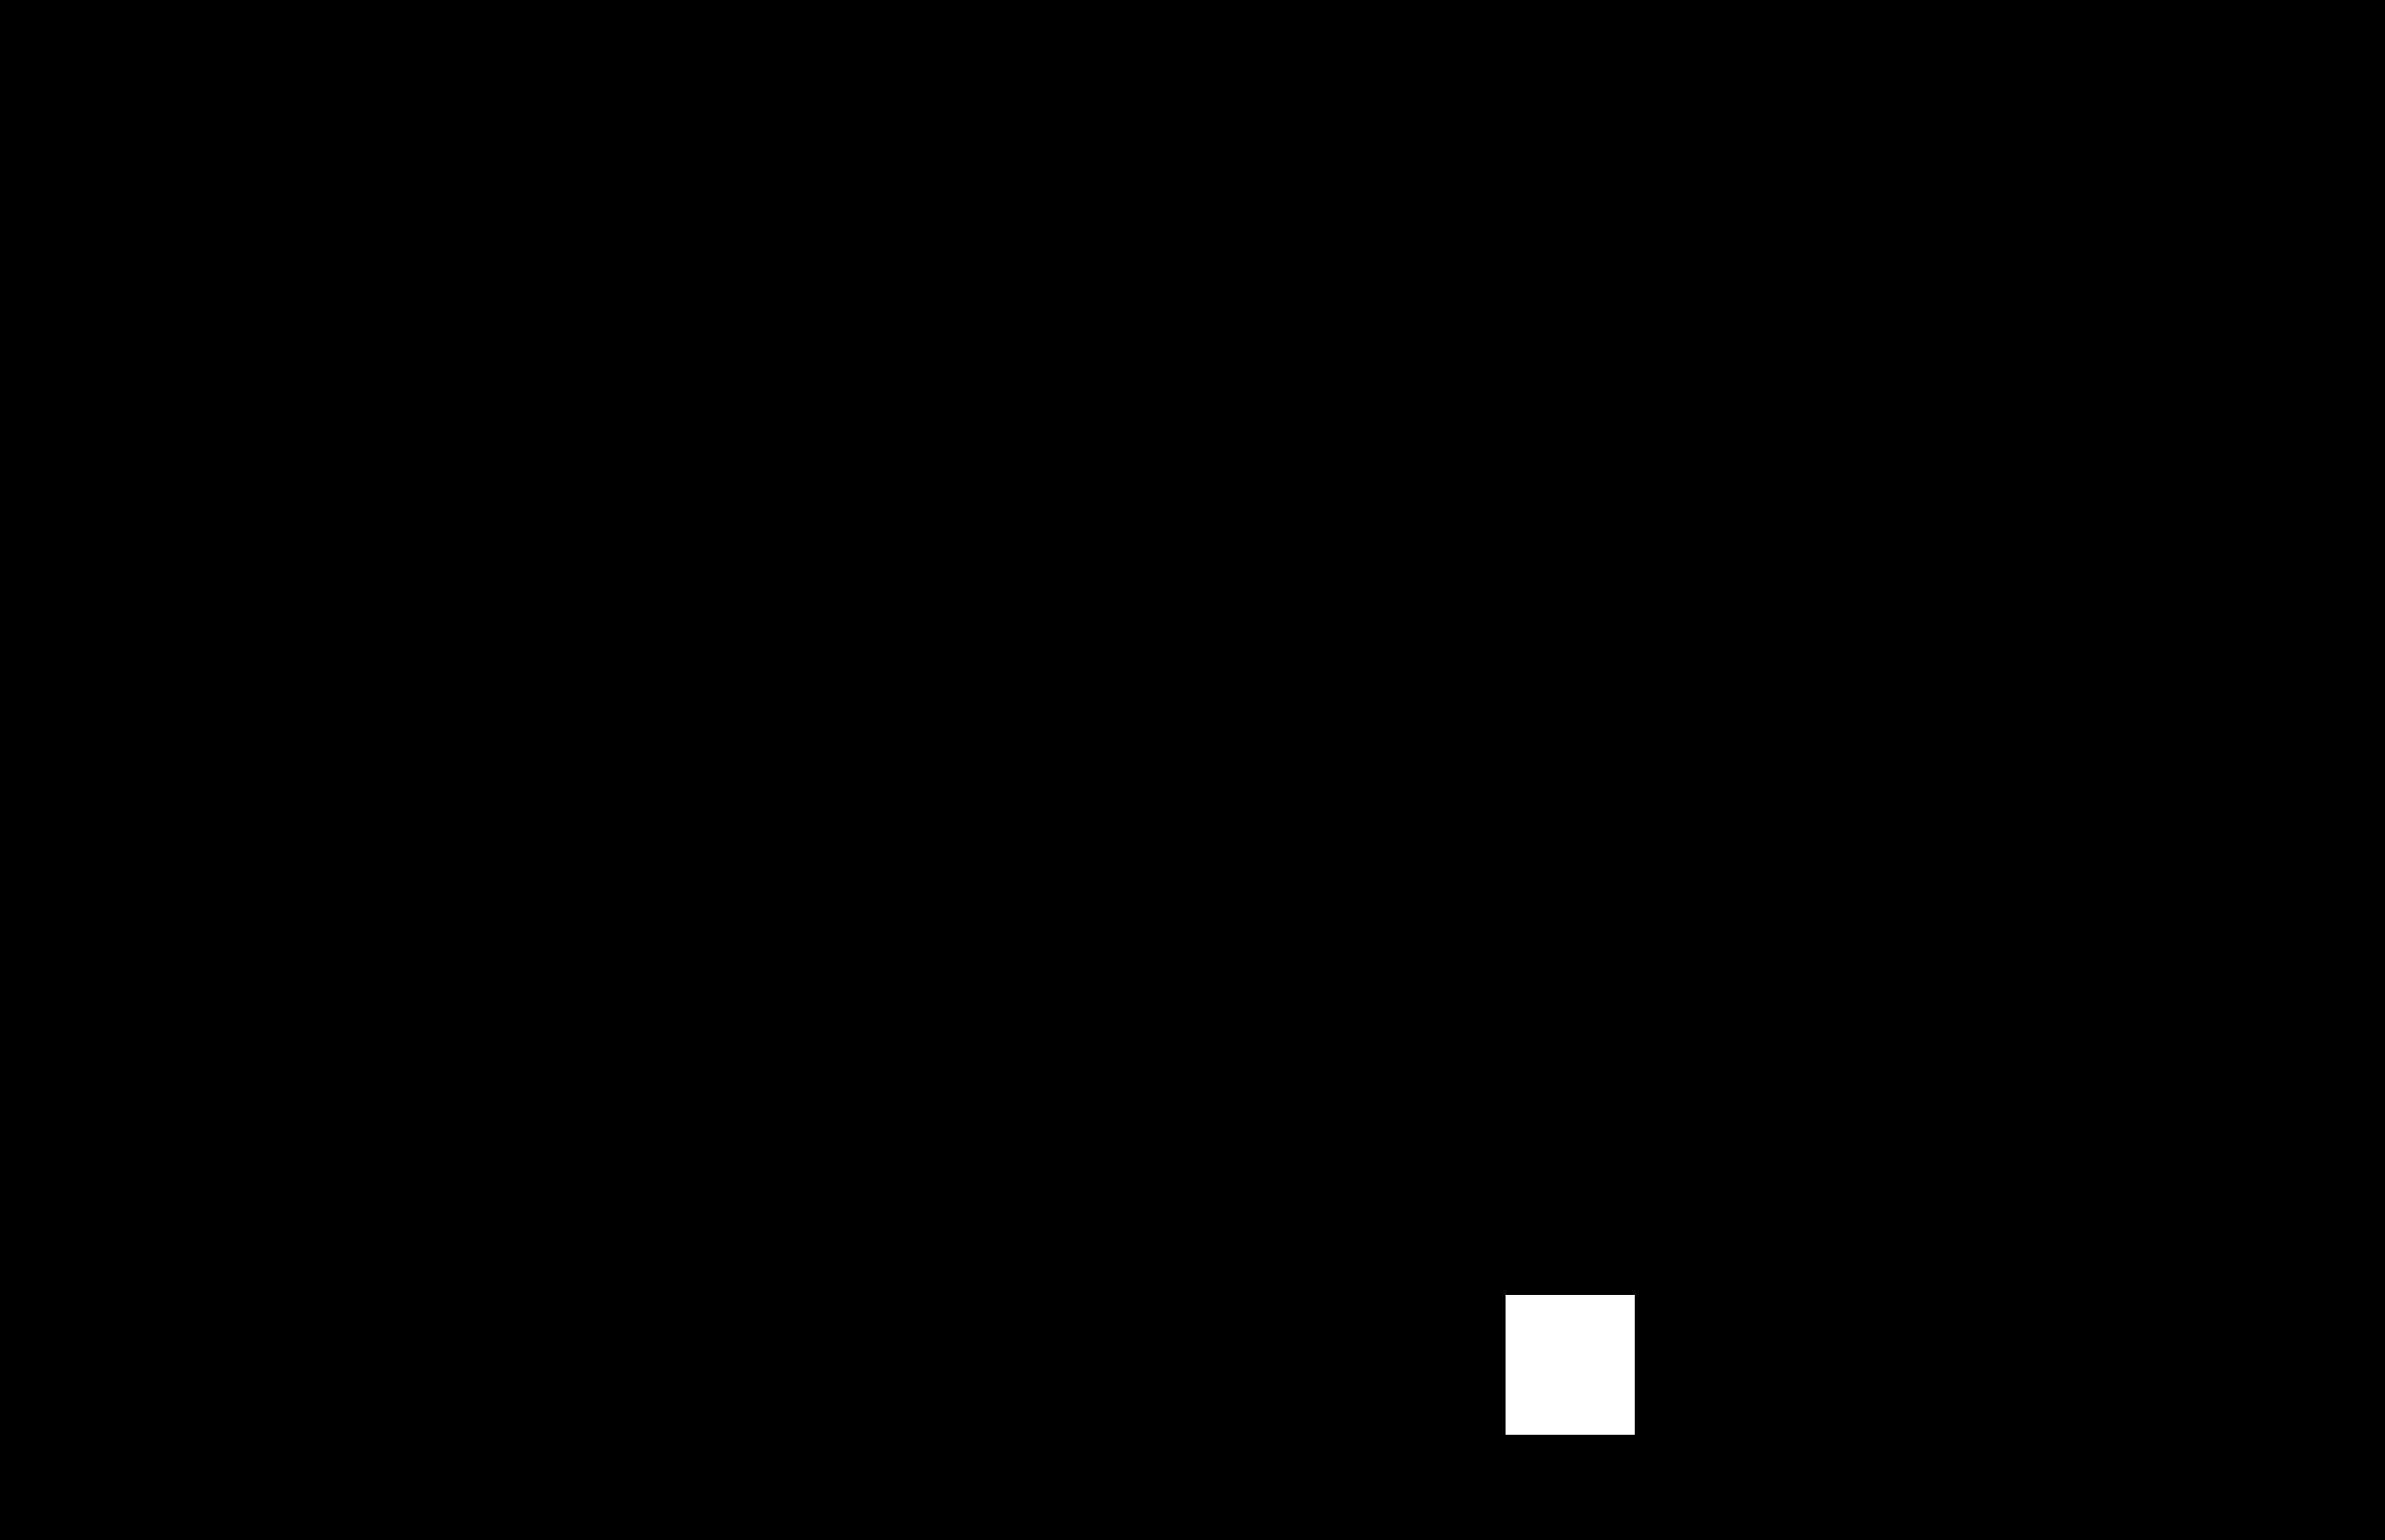
\includegraphics[width=6.6cm]{pipeline/tic_assignee_mask1.jpg}}}%
    \caption{Image and its ticket assignee mask}%
    \label{fig:assignee_masks}%
\end{figure}


\chapter{Workflow}
\section{Launch}
The application is easy to instantiate. The first step is to add the API token for your Todoist account in the settings file of the application. The second step is to launch the mongoDB instance through the \textit{src/db\_start.sh} script. And finally, the application itself is launched through the \textit{src/run.sh} script.
\section{Customizability}
The CV aspect of the application, the specific file names used, the board color, the grid color and the minimum sizes for different entities can be customized from the \textit{settings.json} file, which is easy to edit, and upon encountering formatting errors, the application throws an exception.

The section mappings are done through the \textit{Sections.json} file, which is a preset template from analyzing the initial image. In it, you can map the various detected sections (which are identified by digits) to section names and the various functions they might have, which are explained in \autoref{sec:finding_sec}. Also, you can have a workflow, which is a regular expression denoting the allowed transitions of a ticket on the board. And finally, you can preset the ticket limits for the sections on the board; an example of such mapping is given in listing \ref{lis:sections}.

\newpage
\begin{lstlisting}[language=json,firstnumber=1,caption={Sections.json},captionpos=b]
{
    "map_string" : {
        "1" : "backlog", 
        "2" : "final",
        "3" : "frontend_doing",
        "4" : "frontend_testing",
        "5" : "doing_limit",
        "6" : "none"
    },

    "regex" : "(backlog-)|(^backlog-backend_doing-)(backend_doing-|backend_testing-)*(backend_testing-|backend_testing-final-)?|(^backlog-frontend_doing-)(frontend_doing-|frontend_testing-)*(frontend_testing-|frontend_testing-final-)?",

    "doing_limit" : 1,
    "testing_limit" : 2,
    "backlog_limit" : 3
}
\end{lstlisting}
\label{lis:sections}

\section{Performance}
The program is meant to capture the changes on the board when there is nobody in front of it. For this process to even be feasible, 2 conditions need to be true:

\begin{enumerate}
    \item The images need to be taken often enough to capture every change on the board, meaning that only a single action should need to be performed on a ticket within the capture time window of the camera.
    \item The processing needs to be quick enough to interpret the changes from the previous frame and to make the change on the project management service.
\end{enumerate}

It is reasonable to assume that a ticket on a development team takes at the minimum 10 minutes to complete and that one person can make a change to a given ticket at a time, so making singular changes to multiple tickets in the same cycle does not cause any problems. 

\subsection{Processing speed}
The processing times are displayed in \autoref{tab:process}. It should be noted that detecting when the board is obstructed is very quick, and the program automatically discards the image, instead if trying to do any further processing. However, once the board is detected, there is a 3-second processing cost of trying to find the changes.

\begin{table}[h]
    \centering
    \begin{tabular}{|l|l|}
    \hline
    \textbf{Action}           & \textbf{Processing Time} \\ \hline \hline
    Board is obstructed       & 1 second                  \\ \hline
    No changes detected       & 4 seconds                 \\ \hline
    Single change detected    & 5 seconds                 \\ \hline
    Multiple changes detected & 5-7 seconds               \\ \hline
    \end{tabular}
    \caption{Processing time table}
    \label{tab:process}
\end{table}

All of this leads to the conclusion that a 20 second period between photographs is a reasonable amount, as it isn't expected that a singular entity, be it a ticket or assignee tag, will change more than once in that time frame, and it is more than enough to process any changes that could happen.
\subsection{RAM usage}
The RAM usage of the application is \textit{O(r(s+t))}, where \textit{r} is the number of pixels in the image (resolution), \textit{s} is the number of sections on the board and \textit{t} is the number of tickets on the board. That is because the board stores and uses the ticket and section masks at full resolution. Although directly from the camera the images are up to 5MB, the masks are up to 1MB in Python, as they are binary\footnote{Contain only black and white.}.

\section{Visualization}
It was necessary to create a unique solution for visualizing the changes which are happening on the board between frames. This was for receiving feedback, validating results and testing. Given that this is a computer vision research project, unit testing would not be able to validate the results.

\begin{table}[h]
    \centering
    \begin{tabular}{|l|l|l|l|} 
    \hline
    \textbf{Entity}           & \textbf{Action}                                                                                  & \textbf{Graphic Type}  & \textbf{Color}                        \\ 
    \hline \hline
    \multirow{9}{*}{Ticket}   & \multirow{2}{*}{moved to section}                                                                & line                   & {\cellcolor[rgb]{0.196,1,0.196}}      \\ 
    \hhline{|~|~|-|-|}
                              &                                                                                                  & border                 & {\cellcolor[rgb]{0.118,1,0.118}}      \\ 
    \hhline{|~|-|-|-|}
                              & moved illegally to section                                                                       & line                   & {\cellcolor{red}}                     \\ 
    \hhline{|~|-|-|-|}
                              & removed from section                                                                             & border                 & {\cellcolor[rgb]{1,0.784,0}}          \\ 
    \hhline{|~|-|-|-|}
                              & removed from final section                                                                       & border                 & {\cellcolor[rgb]{0.275,0.353,0.275}}  \\ 
    \hhline{|~|-|-|-|}
                              & \multirow{2}{*}{\begin{tabular}[c]{@{}l@{}}duplicate found in\\ different section \end{tabular}} & line                   & {\cellcolor[rgb]{1,0.686,0}}          \\ 
    \hhline{|~|~|-|-|}
                              &                                                                                                  & border                 & {\cellcolor[rgb]{1,0.686,0}}          \\ 
    \hhline{|~|-|-|-|}
                              & not found in database                                                                            & border                 & {\cellcolor[rgb]{0.784,0,0.784}}      \\ 
    \hhline{|~|-|-|-|}
                              & has multiple assignees                                                                           & border                 & {\cellcolor[rgb]{0.882,0.627,0}}      \\ 
    \hline
    \multirow{3}{*}{Assignee} & assigned to ticket                                                                               & border                 & {\cellcolor[rgb]{0.039,0.353,0.902}}  \\ 
    \hhline{|~|-|-|-|}
                              & not assigned to ticket                                                                           & border                 & {\cellcolor{red}}                     \\ 
    \hhline{|~|-|-|-|}
                              & duplicate across tickets                                                                         & line                   & {\cellcolor[rgb]{0.882,0.627,0}}      \\ 
    \hline
    \multirow{2}{*}{Section}  & limit reached                                                                                    & border                 & {\cellcolor[rgb]{1,0.765,0.176}}      \\ 
    \hhline{|~|-|-|-|}
                              & limit surpassed                                                                                  & border                 & {\cellcolor[rgb]{1,0.392,0.392}}      \\
    \hline
    \end{tabular}
    \caption{Table for graphic change visualization}
    \label{tab:visual}
    \end{table}

The color coding for the change visualizations can be seen in \autoref{tab:visual}. The lines are used for connecting entities on the board, and the borders are rectangles surrounding them, as seen in \autoref{fig:visualized}.

\begin{figure}[h]
    \centering
    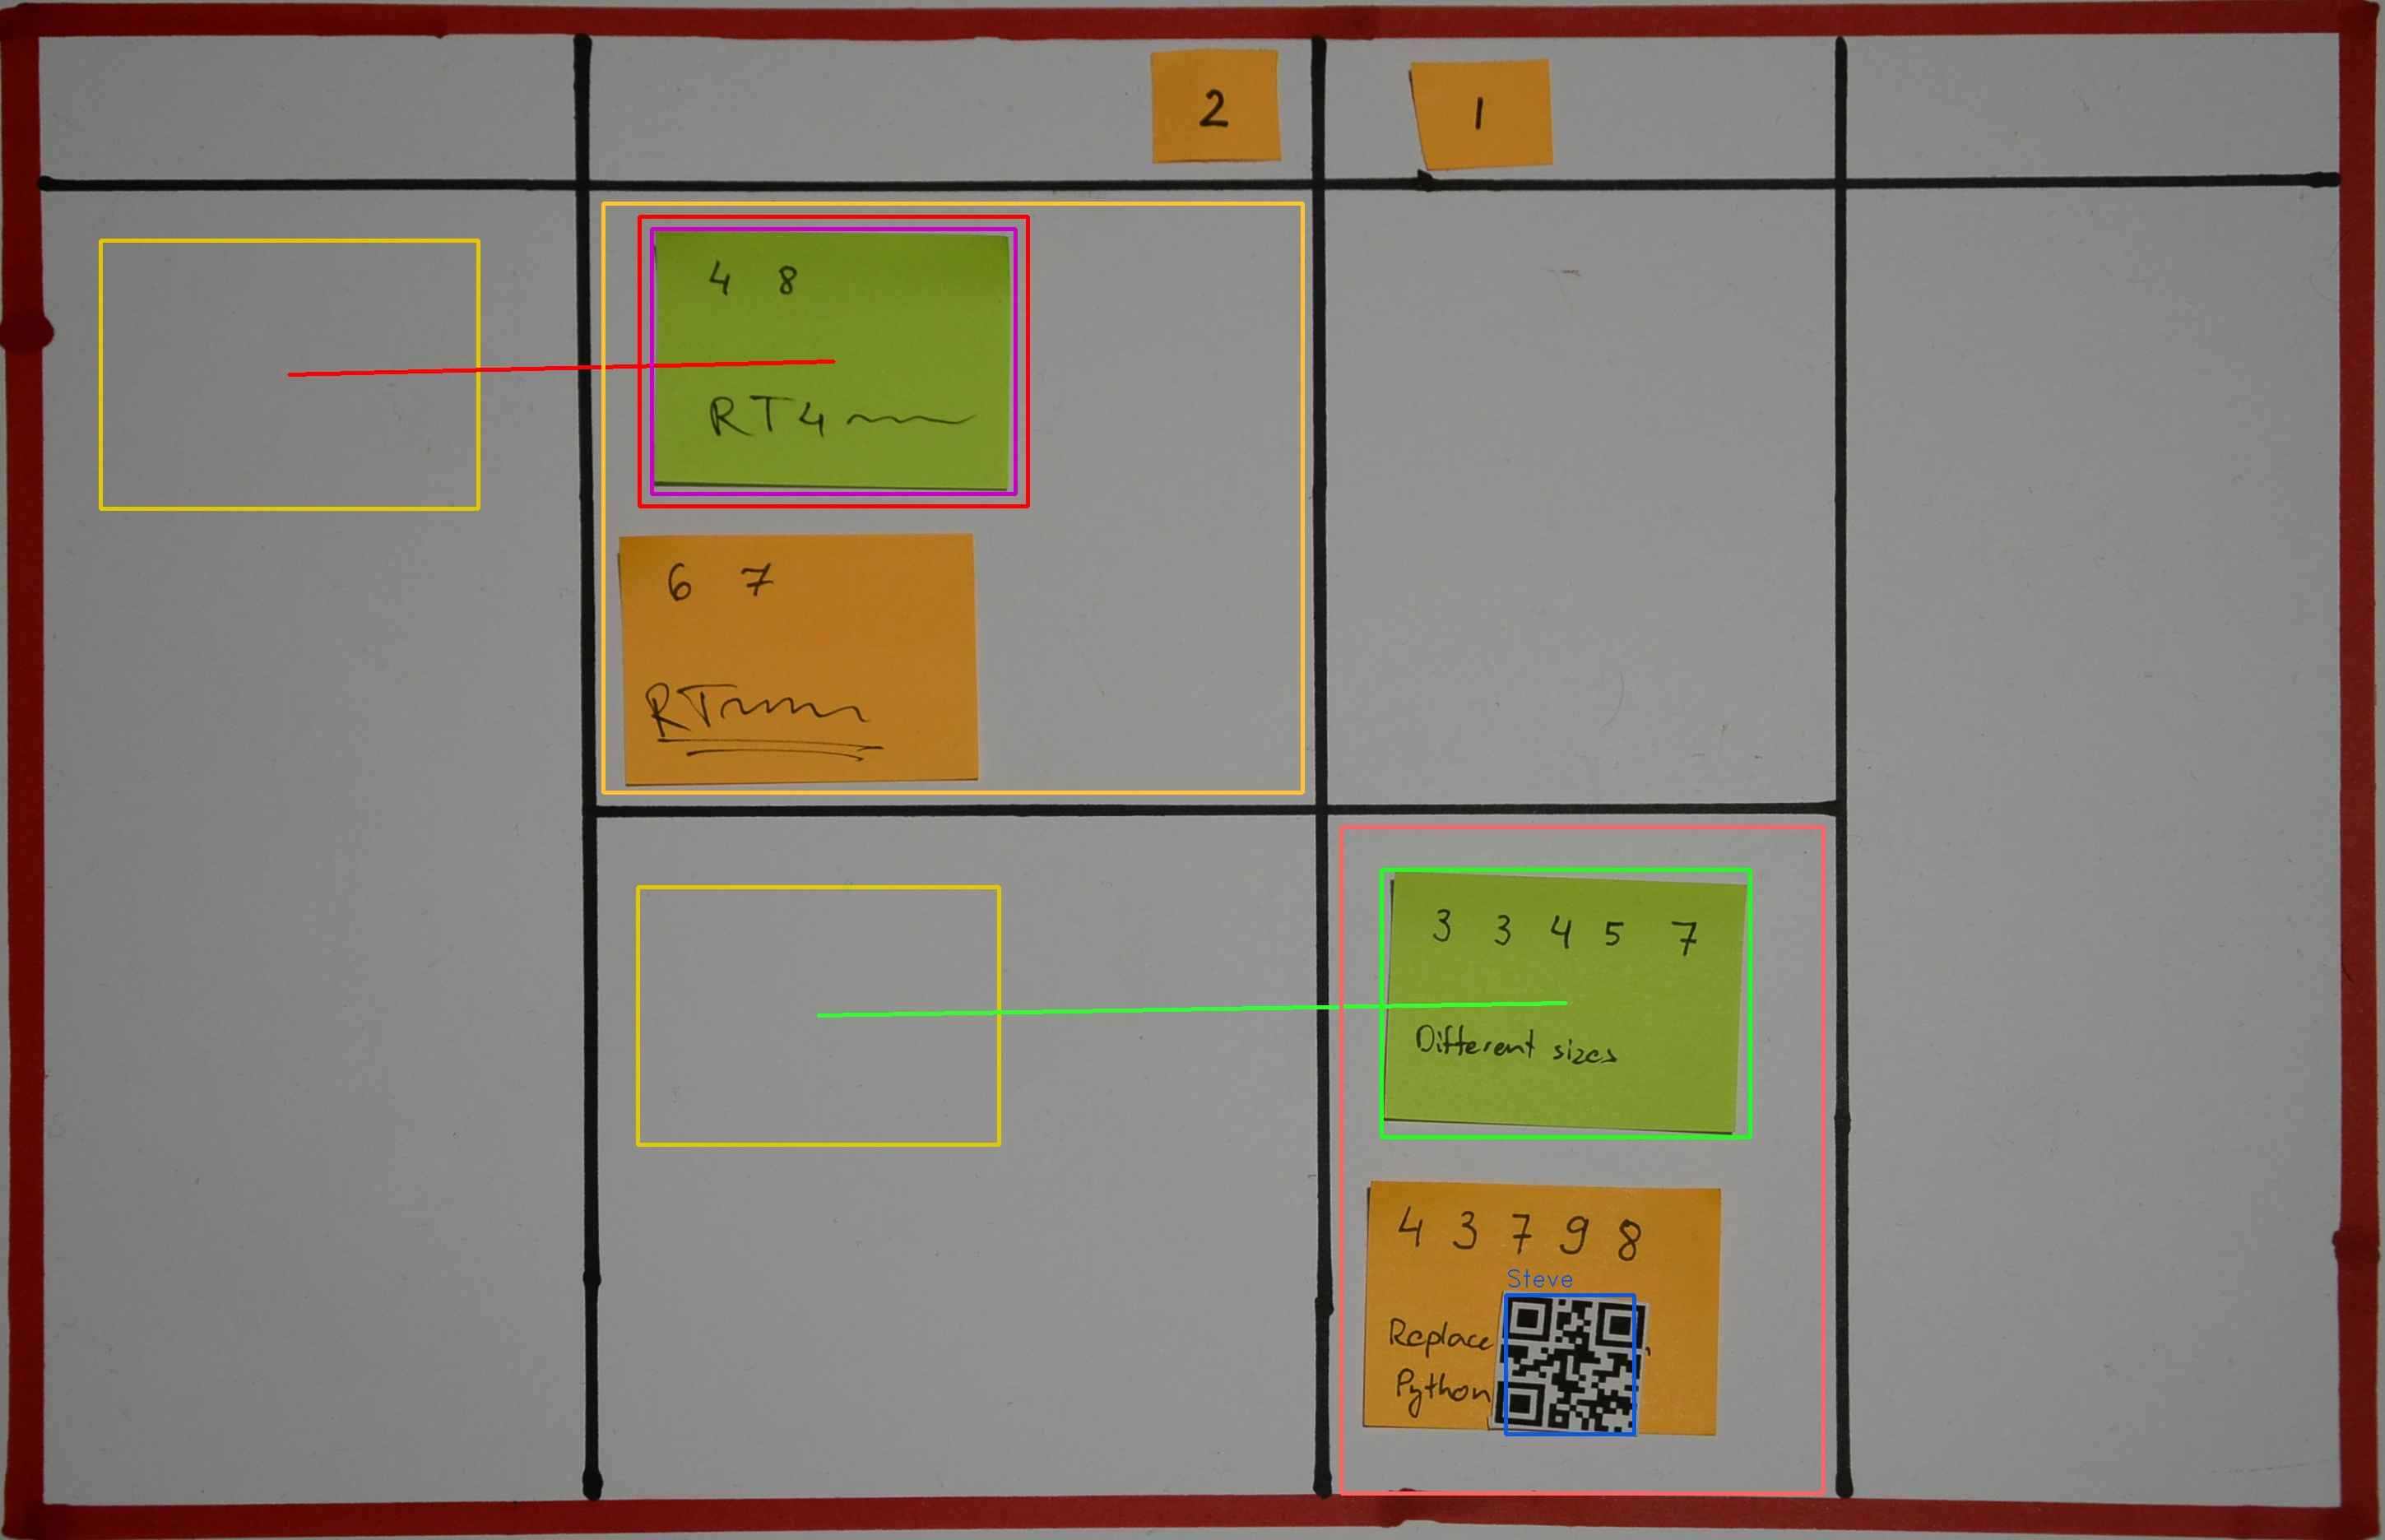
\includegraphics[width=\textwidth]{pipeline/board_extracted.jpg}
    \caption{Visualization of the changes on the board}
    \label{fig:visualized}
\end{figure}

\section{Textual feedback}
The program does not have a graphical interface, only a console one, which lead to the development of workarounds to this deficiency. However, upon using the application it was discovered that a graphical UI might not be necessary at all, as most project management services have their own graphical user interface.
\subsection{Logging}
Logging serves as a communication layer between the users of a program and the system administrator who supervises it. It is used to inform the administrator of the current state the system exhibits, and more importantly to alert them of any erroneous behavior in the system.

A log file records either events that occur in an operating system or other software runs \cite{logging}. Logging packages allow the programmers to customize what level of importance the messages should possess before being recorded. The different messages output by the application along with their logging levels are outlined in \autoref{tab:logginglvls}.

\subsection{ASCII}
This interface in \autoref{fig:ascii} was only used for demo purposes and the library used to draw it is \textbf{terminaltables}\footnote{\url{https://github.com/Robpol86/terminaltables}}, which can be installed through PIP.

\begin{table}[h]
    \centering
    \begin{tabular}{|l|l|l|}
    \hline
    \multicolumn{1}{|c|}{\textbf{Level}} & \multicolumn{1}{c|}{\textbf{Target}} & \multicolumn{1}{c|}{\textbf{Purpose}}                                                                                                                                                                                                         \\ \hline \hline
    DEBUG                                & Developers                           & aid in development                                                                                                                                                                                                                            \\ \hline
    INFO                                 & Users                                & \begin{tabular}[c]{@{}l@{}}inform of ticket movement\\ inform of ticket assignments\\ inform of section limit changes\\ inform of section limits being reached\\ inform of API operations\end{tabular}                                        \\ \hline
    WARNING                              & Users                                & \begin{tabular}[c]{@{}l@{}}warn about incorrect ticket movements\\ warn about section limits being reached\\ warn about section limits being surpassed\\ warn about multiple assignments\\ warn about the board being obstructed\end{tabular} \\ \hline
    ERROR                                & Project Manager                      & \begin{tabular}[c]{@{}l@{}}alert of tickets not existing in the database\\ alert of section limits being surpassed\\ alert of database connection timeouts\\ alert of API connection timeouts\end{tabular}                                    \\ \hline
    CRITICAL                             & Project Manager                      & not used                                                                                                                                                                                                                                      \\ \hline
    \end{tabular}
    \caption{Logging output in the console of the application}
    \label{tab:logginglvls}
\end{table}

\begin{figure}[h]
\begin{verbatim}
+----+----------+------------------+-------+-------------------+
| ID | Function | Name             | Limit | Tickets           |
+----+----------+------------------+-------+-------------------+
| 1  | TICKET   | backlog          | 3     | 48 :  ([])        |
|    |          |                  |       | 67 : RT --- ([])  |
+----+----------+------------------+-------+-------------------+
| 2  | FINAL    | final            | 100   |                   |
+----+----------+------------------+-------+-------------------+
| 3  | TICKET   | backend_doing    | 1     |                   |
+----+----------+------------------+-------+-------------------+
| 4  | TICKET   | frontend_doing   | 1     |                   |
+----+----------+------------------+-------+-------------------+
| 5  | TICKET   | backend_testing  | 2     |                   |
+----+----------+------------------+-------+-------------------+
| 6  | TICKET   | frontend_testing | 2     |                   |
+----+----------+------------------+-------+-------------------+
\end{verbatim}
\caption{ASCII interface}
\label{fig:ascii}
\end{figure}

\chapter{Communication Layer}
Of significant importance to the success of the project was the one-way communication of the program with a third party API. With the inclusion of an API, came the management of auto-generated IDs at each individual run of the program. Those IDs could have been part of the python objects, but architecturally, there needed to be a decoupling of the communication layer and the computer vision portion. The inclusion of mongoDB wasn't pivotal to the overall success of the implementation, however, the interface proved to be reliable and fast, and additionally provided some much-needed separation in logic, so it made it to the latest version.

\section{mongoDB}
MongoDB is a highly scalable and agile NoSQL database, which is a mechanism for storage and retrieval of data unlike that of relational database management systems. NoSQL offers high performance with high availability and offers rich query language and easy scalability \cite{nosql}.

The choice to use a NoSQL solution was an easy one; there is only a single relationship - from the sections to the tickets, and the database didn't necessarily need to model it, which is the strong point of relational databases. The process of interfacing in SQL is more complex, which would have only penalized development, as the program was not designed to utilize its schema, normalization, and bulk retrieval benefits.

\begin{figure}[h]
    \centering
    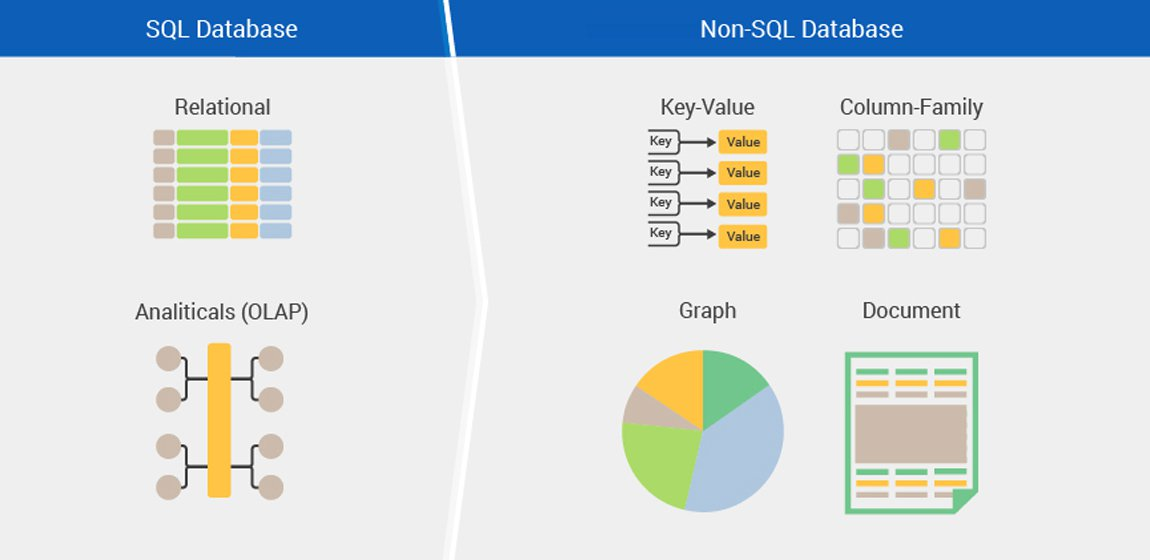
\includegraphics[width=\textwidth]{img/stock/sql_vs_nosql.JPG}
    \caption{SQL and NoSQL}
    \label{fig:sql_vs_nosql}
\end{figure}


From the project planning stage, the project was designed around the possibility of including mongoDB - it being a cross-platform document-oriented database program, with strong community support and reliable local hosting. MongoDB uses JSON-like documents natively for storing the records, and being built in C++ made it a strong contender, given that speed was of great importance. 

It was preferable for the database interface to support JSON, which was already heavily embedded into the architecture of the project, so mongoDB's direct support for JSON in querries simplified the translation of changes. The lack of SQL notation did not pose a problem, as the application was only meant to deal with direct changes, relying on mongoDB's \textit{find\_one} method syntax.

\section{Todoist}
Todoist was the application chosen for interfacing due to its documentation, the established community around it and its popularity. It has a simple interface, supported the creation, editing of tasks and moving those tasks across projects. It also permitted creating subprojects, which structured them conveniently for the project's use.

While the application is not the clearest choice for a task board representation, it provided sufficient functionality and a possessed a consistent visual language for making changes and warnings explicit.


\chapter{Conclusion}
\section{Reflections}
The project has succeeded in delivering more functional requirements than initially expected, as well as capturing some of the non-functional ones. The few things missing from it are a robust user-friendly interface and the actual live transmission of photos from the camera to the program. Given the forgoing of those features, the focus of the project was shifted towards examining the feasibility of a system with the desired properties, that being: change detection, digit recognition, ticket assignments, and general section detection.

Initially, the plan for the project was to create a separate web service which would host the captured images, containing the extracted data and the captured changes. However, once a method for automating section segmentation was found, the need for such an interface became less apparent, and thus resources were contributed to the polishing the key aspects of the project.

An attempt at photo transmission was made using the application \textbf{Time Lapse to Cloud}\footnote{\url{https://tinyurl.com/time-lapse-to-cloud
}}, however after thorough experimentation, it was found that the camera of the OnePlus 5T\footnote{\url{https://www.oneplus.com/uk/oneplus-5t}} did not produce sharp enough images for the program to recognize the digits that the tickets carried. Although the concept of piping a time lapse output from \textbf{Google Drive}\footnote{\url{https://www.google.com/drive/}} to the program through a bash script was successful, ultimately the idea was scrapped due to the hardware limitations of the small image sensors found on the smartphone.

\subsection{Development progression}

The project development actually began in October, without much overlap in feature development at the beginning. From the Gantt chart in \ref{fig:gantt} it is noticeable that the board detection, section segmentation and overall structuring of the project were very self-contained, and were done separately in succession. Although those features took roughly as long to develop as the rest of the feature set, they served as a foundation for the overall consistency of the frame-to-frame CV operations.

\begin{figure}[h]
    \centering
    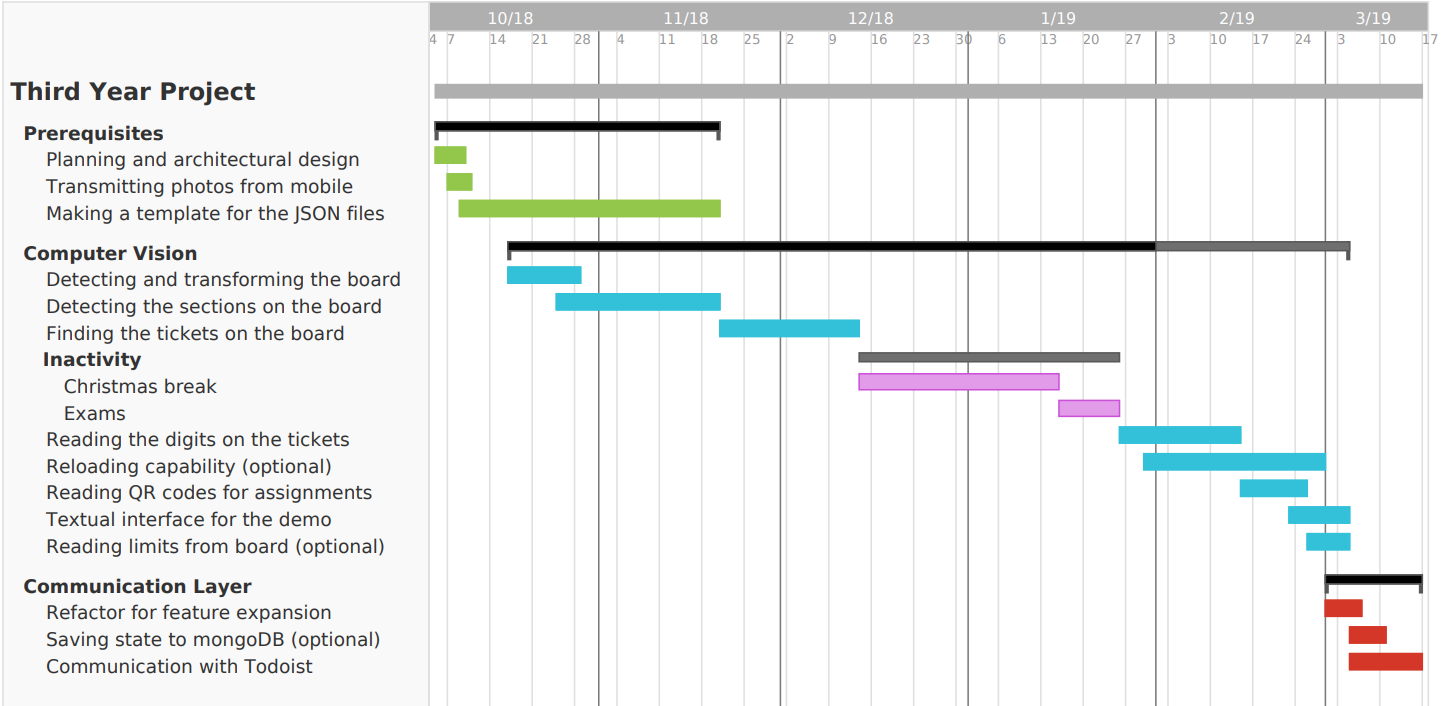
\includegraphics[width=\textwidth]{img/gantt_chart.png}
    \caption{Project progress Gantt chart}
    \label{fig:gantt}
\end{figure}

Detecting the tickets and reading the digits from them were the most time-consuming tasks, and posed the greatest difficulty. Mere differentiation would cause a lot of noise, and the nature of the JPG format posed a significant threat to the success of the project.

There was a trial and error element to finding methods of block detection with ticket differentiation that would serve the project, some of which being KNN color classification for the board color and the ticket colors, which for time consuming to train, slow for classification and yielded inconsistent results. SVM training, while faster, was also inconsistent in its classifications.

The post-exam period was the most productive, and as seen in \ref{fig:gantt}, the implementation of a fully functioning digit detection and classification method kick-started the rest of the crucial feature development. A couple of features were implemented with the in-person demonstration in mind, which was on March 6, examples being the limit detection and the reloading capabilities.

The final period was post-demo, and it was putting everything together to function as part of an established service. With the bulk of the project done and the proof of concept established, there was bound to be some refactoring done to be able to easily incorporate the communication layer. While the last few weren't the ones which make or break the project, they were a valuable addition to the overall user experience.



\subsection{Development choices}
One of the defining choices for the project was using Python as opposed to C++ for interfacing with OpenCV. With the purpose of the project being demonstrating feasibility, Python was the language of choice due to its versatility in smaller scale projects. The calculations were mostly done using NumPy and OpenCV, both of which are Python wrappers for underlying C++ code, which meant that the system could both benefit from the simplicity of Python and the speed of C++ \cite{array_manipulation}, the only small penalty being the calls to the C++ code itself were being done in Python, and as an interpreted language, it was bound to be slower than a pure C++ solution.

Portability and dependency management also played a role in choosing Python over C++. Given that the requirements from the \textit{requirements.txt} are loaded into the Python virtual environment beforehand, the project should function unconditionally. All of the dependencies could individually be downloaded using PIP, which is available for Linux, macOS, and Windows.

An aspect of the method itself that could be improved is its flexibility. The border itself, for example, needs to be of a solid color, which is predefined using HSV values for its brightest and darkest limits. If the lighting were to change (e.g. from incandescent to natural light), these values do not hold as well. The problem with tickets that don't have strongly distinguishable colors is a serious one, and it would involve a more complex solution than hard-coded thresholds, involving machine learning for classifying lighting conditions.

\section{Future work}
While there are no plans of expanding the project, given it was treated as a research experiment as opposed to a finalized solution. Image differentiation and color classification are both branches of image processing that could greatly improve the performance and reliability, but their inclusion would need a complete rewrite of the project.

The application was developed with parallelization in mind, and although it does not implement it, the operations are not strictly serial. The differentiations with the previous image and with the background image could run in parallel, as well as the digit classifications for the individual tickets, as they are the most expensive operations. Utilizing the multi-core capabilities of modern CPUs could be done using the \textbf{multiprocessing}\footnote{\url{https://docs.python.org/2/library/multiprocessing.html}} Python library, which would allow bypassing its \textbf{Global Interpreter Lock} \cite{multiproc}.
\section{Summary}
The project successfully demonstrates that it is possible to interpret a task board from consecutive photographs, given a high enough resolution, static lighting and controlled interaction with the board. Using simple string matching, it is able to map the tickets on the board precisely to the ones found in the database and make the changes accordingly with each iteration.

The program can reliably find a board in the scene, assign sections to their names and roles, as well as utilize those mappings in an instinctive manner for a software developer. The different interfaces present the changes from state to state in a clear and easy to understand manner, without compromising on speed of execution. The program can capture many correct and a few undesirable interactions with the board, and communicate any errors with the user. It is able to detect changes from frame to frame, assignments of tickets to users, changes in limits of sections, and inform of any changes which are not in accordance with the preset rules.

While the original premise was clear from the planning stage, the complexity of the decisions at each incremental step only unfolded when development was underway. The level of human error which can be introduced when simply interacting with a physical object is beyond what a single developer could ever hope to account for. Tickets could intersect, be placed upside down, be put at an odd angle, and even have numbers with written using irregular handwriting. If a person struggles to recognize a digit, how could they expect OCR software to predict it? The element of randomness makes the project unfeasible in a real-world use. Given that ideally, it would use only the titles of the tickets, instead of numbers, the issue of handwriting becomes even more pressing.

Considering the above, combined with the impracticality of having a permanently stationed camera in an office environment, the only solution to the problems in \ref{subsec:problems} is to only have a fully digital board, which emulates the physical one and is directly synchronized with or embedded in the project tracking software.

\bibliographystyle{ieeetr}
\bibliography{references.bib}

\end{document}
